\documentclass[a4paper,11pt,twoside]{book}
%\documentclass[11pt,twoside,letterpaper]{book}
\usepackage{a4wide}
%\usepackage{multirow}
\usepackage{footnote}
\usepackage{amsbsy}
\usepackage{amsmath}
\usepackage{amssymb}
\usepackage{gensymb}
\usepackage[dvips]{graphicx}
%\usepackage{fancyheadings}
\usepackage{fancyhdr}
\usepackage{nicefrac}
%\setlength{\parindent}{0in}
%\setlength{\parskip}{0.05in}
\setlength{\parskip}{0.1in}
\bibliographystyle{plain}
%\usepackage{a4wide}
\usepackage{color}
\def\red{\textcolor{red}}
\usepackage{lscape}

\usepackage{hyperref}

%\parskip=2mm
\newcommand{\kbf}{\mathbf{k}}
\renewcommand{\d}{\mathrm{d}}
\newcommand{\e}{\mathrm{e}}

% Ensure that blank pages don't have numbers or heading on them
\makeatletter
\def\cleardoublepage{\clearpage\if@twoside \ifodd\c@page\else
 \hbox{}
 \vspace*{\fill}
 \thispagestyle{empty}
 \newpage\fi\fi}
\makeatother

% set fancy headings
\pagestyle{fancy}
\lhead[{\it \thepage}]{{\bf\it {\tt OptaDOS}: User Guide}}
\chead{}
\rhead[{\bf\it {\tt OptaDOS}: User Guide}]{{\it \thepage}}
\renewcommand{\headrulewidth}{0.2pt}
\lfoot{}
\cfoot{}
\rfoot{}
\renewcommand{\footrulewidth}{0pt}
\setlength{\footskip}{0.25in}
\setlength{\parindent}{0in}



\title{{\huge {\tt OptaDOS}: User Guide}\\ {Version 1.3.388}}

\author{Andrew J. Morris, Rebecca J. Nicholls, Chris J. Pickard, Jonathan R. Yates \\
\\
Department of Metallurgy and Materials\\
University of Birmingham \\
Elms Road\\
Edgbaston\\
Birmingham\\
UK\\
%Department of Physics\\
%University of Cambridge\\
%19 J.~J. Thomson Ave\\
%Cambridge CB3 0FF\\
%UK,\\
\\
Department of Materials\\
University of Oxford\\
Parks Road\\
Oxford\\
UK \\
\\
{\small and} \\
\\
Department of Materials Science and Metallurgy\\
University of Cambridge\\
27 Charles Babbage Rd\\
Cambridge\\
UK\\
%Department of Physics and Astronomy\\
%University College London\\
%Gower Street\\
%London WC1E 6BT\\
%UK}
}


\date{February 2019}

\begin{document}
\newcommand{\optados}{\textsc{OptaDOS}}
\newcommand{\lindos}{\texttt{LinDOS}}
\newcommand{\onetep}{\textsc{onetep}}
\newcommand{\castep}{\textsc{castep}}
\newcommand{\python}{\textsc{Python}}
\maketitle

%%%%% Copyright page
 \thispagestyle{empty}

\begin{centering}
\vspace*{40mm}
University of Cambridge, University of Oxford and University College London\\
\vspace{5mm}
\copyright\ 2013-2022 A.~J. Morris, R.~J. Nicholls, C.~J. Pickard and J.~R. Yates.\\
\vspace{5mm}
First published 2010\\
This edition 2019\\
\vspace{5mm}
10 9 8 7 6 5 4 3 2 1
\vspace{5mm}

Part of this work published in:\\
``OptaDOS: A Tool for Obtaining Density of States, Core-loss and Optical Spectra from Electronic Structure Codes'', Andrew J. Morris, Rebecca J. Nicholls, Chris J. Pickard and Jonathan R. Yates, Comp. Phys. Comm. {\bf 185}, 5, 1477 (2014)\\
\vspace{10mm}
Further information about \optados\ may be obtained from:\\ \texttt{www.optados.org}\\

\vspace{10mm}
\emph{Nota bene:} \optados, optados or OptaDOS, but never OPTADOS.

\null\vfill
\noindent
Font: Computer Modern, 11pt\\
Typeset by the authors using \LaTeX\, \\
\end{centering}
\newpage

\setcounter{tocdepth}{1}
\tableofcontents

\newpage
 \thispagestyle{empty}
\vspace*{50mm}
\begin{centering}
We would like to thank Phil Hasnip and Keith Refson for very helpful discussions and Gareth Griffiths and Kane O'Donnell for extensive beta testing.
 AJM, RJN and CJP acknowledge support from the EPSRC. Additionally AJM acknowledges
the Winton programme for the physics of sustainability and RJN the ERC
(Grant ERC-2009-StG-240500).
 JRY acknowledges support from the Royal Society through a University Research fellowship.
\end{centering}
\begin{flushright}
AJM, RJN, CJP and JRY\\
September 2013
\end{flushright}

\chapter*{Contributors}
 \thispagestyle{empty}

\begin{itemize}
\item Matthew L. Evans, University of Cambridge: projected bandstructures and bug fixes.
\item Angela F. Harper, University of Cambridge: Mizoguchi chemical shift for coreloss calculations.
\end{itemize}

\chapter{Introduction}\label{chap:introduction}
\section{Background}
\optados\ is a code for calculating optical, core-level excitation spectra along with full, partial and joint electronic density of states (DOS).  The code was developed by merging the \lindos\ code of Andrew Morris and Chris Pickard at University College London with the optical properties code of Rebecca Nicholls and Jonathan Yates at Oxford University.  \optados\ is written in Fortran 95 and may be run in parallel using {\tt MPI}.  At present \optados\ interfaces with \castep\ and \onetep\ output files, although it is extendible to perform calculations on any set of band eigenvalues and their derivatives generated by any electronic structure code.

The code is freely available through the GPL licence with the request that the following citation (quoted in full) is required in any publication resulting from the use of \optados.

\emph{Andrew\,J. Morris, R.\,J. Nicholls, C.\,J. Pickard and Jonathan\,R. Yates, \optados: A Tool for Obtaining Density of States, Core-level and Optical Spectra from Electronic Structure Codes,  Comp. Phys. Comm. {\bf 185}, 5, 1477,(2014)}

\begin{center}
Further information and examples can be found at

\verb#www.optados.org#
\end{center}


\section{Features}
\optados\ generates optical, core-level excitation spectra along with full, partial and joint electronic DOS. The DOS, PDOS and JDOS take advantage of the linear and adaptive broadening schemes which are more accurate than standard Gaussian broadening since they exploit knowledge of the gradients of the bands at each $k$-point in the Brillouin zone.  These DOS are the basis of the more advanced functionality of \optados, the core and optical spectra.

Along with data text files \optados\ also generates \verb#.agr# files of results to be read by \verb#grace#.




%%%%%%%%%%%%%%%%%%%%%%%%%%%%%%%%
\chapter{Theoretical Background} \label{sec:theory}
%%%%%%%%%%%%%%%%%%%%%%%%%%%%%%%%

\section{Integrals over the Brillouin Zone}

Many energy-resolved spectral properties of a material take the form of an integration of some function, $F_{nm}(\kbf)$ in  reciprocal space over the BZ; where $F_{nm}(\kbf)$ are the elements of a periodic operator which commutes with the crystal translational symmetry.
%
Perhaps the two simplest examples of integrals, hereinafter referred to as type (a) and type (b), take the form at T$=0\,$K of,
\begin{equation}
I^{(a)} \left ( E \right) = \sum_n \int_{\rm BZ} \frac {\d\kbf}{(2\pi)^3} F_{nn}(\kbf) \delta (E_{n\kbf}-E),
\end{equation}
and,
\begin{equation}
I^{(b)} \left ( E \right) = \sum^{\rm occ}_n \sum^{\rm unocc}_m
\int_{\rm BZ} \frac {\d\kbf}{(2\pi)^3} F_{nm}(\kbf) \delta ( E - (E_{m\kbf}-E_{n\kbf})),
\label{Eqn:IntB}
\end{equation}
where $E_{n\kbf}$ are the energy eigenvalues of the system.
%
They are also extendible to integration over spin-polarised channels
in a straightforward way.

\section{Brillouin Zone Sampling Schemes}

Since the crystal momentum, $\kbf$, is a continuous quantum number the band structure in an \emph{ab initio} calculation is approximated using specific $k$-points within the first Brillouin zone.
%
These $k$-points may be chosen through symmetry perhaps using a Monkhorst-Pack grid \cite{monkhorst:PRB:1976} or  the multi-$k$-point generalisation to the Baldereschi scheme\cite{rajagopal:PRL:1994,morris:PRB:2008}.


Obtaining the energy bands from a set of eigenenergies at discrete $k$-points is non-trivial.
%
This simplest way of assigning bands, by counting eigenvalues at $k$-points, implicitly assumes that there are no band crossings in the BZ.
%
This is further complicated by ``band kissing'' where bands approach, but due to small interactions between the bands breaking the degeneracy they remain continuous\cite{blochl:PRB:1994,pickard:PRB:1999}.
%
Considering band coefficients and the overlap matrix it has been shown how to assign bands to individual eigenenergies\cite{yazyev:PRB:2002,refson:o2b}, however these still require a broadening scheme to obtain a DOS.
%
Below we detail some approaches to obtaining a DOS from a set of eigenenergies.



\subsection{Gaussian broadening}
%
The reciprocal space is discretised into \emph{sub-cells} each containing a $k$-point which contributes to the integral corresponding to the energy of the $k$-point at their centre.
%
Band dispersion may be crudely approximated by smearing each sub-cell's contribution by a fixed-width Gaussian function, of some width, $\omega$,
\begin{equation}
\delta (E_{n\kbf}-E) \rightarrow \frac{1}{\omega\sqrt{2\pi}}\exp \left (-\frac{1}{2}((E_{n\kbf}-E)/\omega)^2 \right ).
\end{equation}
This approach requires a large number of $k$-points to converge the DOS since when choosing $\omega$ there is a trade-off between representing the sharp features, such as van Hove singularities\cite{vanHove:PR:1953}  and not introducing spurious oscillations due to the limited $k$-point sampling.
%
The band crossing problem is not present since the bands are modelled as dispersionless.

Fixed-width Gaussian broadening may be chosen  for \optados\ calculations with, \texttt{broadening : fixed}.


\subsection{Interpolative schemes}
In the linear tetrahedron interpolative scheme the BZ is divided into
roughly equal size tetrahedra with the band energy calculated at each
vertex \cite{lehmann:PSS:1972}.
%
The DOS contribution of each tetrahedron is then calculated analytically by linear interpolation.

Linear interpolation suffers from the band crossing problem, since the interpolation always joins the lowest energy bands together, which has the effect of avoiding all band crossing and kissing.
%
The method also does not describe van Hove singularities well since the interpolation is linear.

Higher-order interpolation schemes, such as the quadratic tetrahedron scheme,  have been proposed which converge the singularities more rapidly than the linear scheme  \cite{boon:JPC:1986,methfessel:JPC:1983,methfessel:JPC:1987}, but these still require a high-density $k$-point grid to mitigate the band-crossing problem.


\subsection{Extrapolative schemes}
Extrapolating from each $k$-point rather than interpolating between adjacent points eliminates the band-crossing problem.
%
M\"uller and Wilkins show that for free electron bands the DOS is a smooth parabola when using the extrapolative method and a rough unconverged spectrum with the interpolative approach when using the same $k$-point mesh \cite{muller:PRB:1984}.

The linear extrapolative scheme still does not represent van Hove singularities as well as a second-order approach.
%
Band curvatures may be combined with L\"owdin perturbation theory to extrapolate to higher order \cite{pickard:PRB:1999,pickard:PRB:2000}.

Linear extrapolative broadening may be chosen  for \optados\ calculations with, \texttt{broadening : linear}.


\subsection{Adaptive broadening schemes}
An approximation to linear extrapolation method was proposed by Yates \emph{et al.} \cite{yates:PRB:2007}.
%
Each sub-cell's contribution to the DOS is broadened by a Gaussian function whose width, $\omega$, is proportional to the energy band gradient as its $k$-point.
%
This simple approach removes the spurious oscillations of the fixed broadening whilst maintaining the sharper features.
%
The adaptive broadening scheme was introduced in Ref \cite{yates:PRB:2007} in the context of Wannier interpolation of BZ quantities.
%
However, the scheme is more general that this, and with \optados\ we apply adaptive broadening directly to the quantities obtained from the electronic structure calculation.

Adaptive broadening may be chosen  for \optados\ calculations with, \texttt{broadening : adaptive}.



%%%%%%%%%%%%%%%%%%%%%%%%%%%%%%%%
\section{Density of Electronic States}
%%%%%%%%%%%%%%%%%%%%%%%%%%%%%%%%

When $F_{nm}(\kbf)=1$ the type (a) integral represents the electronic density of states (DOS) at $E$ and the total ground-state energy, $E_{\rm gs}$ is obtained by integrating over the occupied energies,
\begin{equation}
E_{\rm gs} = \int^{E_{F}}_0 I^{(a)}( E; F_{nm}(\kbf)=1) \d E,
\end{equation}
where $E_F$ is the Fermi energy.

The DOS is plotted with \optados\ using the \verb@task : dos@ command.

The partial, or projected DOS (PDOS), $I_{\mu}$ is obtained by projecting the DOS onto local orbitals, $\mu$, at each atomic site\cite{segall:MP:1996}.
%
In this case,
\begin{equation}
F_{\mu n}(\kbf)=\Re \left \{  T_{\mu n}^{\dagger}(\kbf) T_{\nu n}(\kbf) S_{\nu \mu}(\kbf)^{-1} \right \},
\end{equation}
where $ T_{\mu n}(\kbf)= \langle \Psi_n(\kbf)|\phi_{\mu}(\kbf)
\rangle$ are the overlap matrices between LCAO (linear combination of
atomic orbitals) basis, $\phi_{\mu}$ and planewave states, $\Psi_n$, and  $ S_{\mu n}(\kbf)=\langle \phi_n(\kbf)|\phi_{\mu}(\kbf) \rangle$, the overlap matrices of the LCAO basis.

The PDOS is plotted with \optados\ using the \verb@task : pdos@
command.
%
The projection is defined using the \verb@pdos@ keyword as described
in the user manual.

In the case of the type (b) integral when $F_{nm}(\kbf)=1$, we
obtain the joint-DOS, (JDOS), for frequency, $\omega$.
%
The JDOS is plotted with \optados\ using the \verb@task : jdos@ command.



\section{Dielectric response}

Core-level spectra and optical properties are related to the complex dielectric function $\varepsilon_1+i\varepsilon_2$.  Within the random phase approximation, the imaginary part of the dielectric function is
\begin{equation}
\varepsilon_2 \left ( \omega \right ) = \frac{\pi e^2}{\varepsilon_0 \Omega} \frac{1}{q^2} \left | \langle  \psi^c_{\bf k}   |  \e^{-i{\bf q}.{\bf r}} | \psi^v_{\bf k + q} \rangle\right |^2,
\end{equation}
where $e$ is the charge on an electron, $\varepsilon_0$ is the permittivity of free space, $\Omega$ is the volume of the unit cell and {\bf q} is the momentum transfer \cite{dressel}.
Using the dipole approximation, expressing {\bf q} as $q\,\hat{\bf{u}}$ and taking the limit that $q \rightarrow 0$, $\varepsilon_2$ can be written as an integral of type (b),
\begin{equation}
\varepsilon_2 \left ( \omega \right ) = \frac{\pi e^2}{\varepsilon_0 \Omega} I^{(b)}\left ( \hbar \omega \right ),
\label{Eqn:Epsilon2}
\end{equation}
where,
\begin{equation}
F_{nm}(\kbf)= \left | \langle \psi^c_{\bf k}  |  \hat{\bf u}\cdot {\bf r} | \psi^v_{\bf k} \rangle\right |^2.
\label{Eqn:Dipole}
\end{equation}
Most electronic structure codes do not calculate $\langle \psi^c_{\bf k}  |  {\bf r} | \psi^v_{\bf k} \rangle$ directly due to the ambiguity of a position operator in periodic cells.
%
Rather they calculate $\langle \psi^c_{\bf k}  |  {\bf p} | \psi^v_{\bf k} \rangle$, where ${\bf p}$ is the momentum operator, which is trivial in reciprocal space.

Since,
\begin{equation}
{\bf p} = m\dot{r} =\frac{im}{\hbar} [\hat{H},{\bf r}]
\label{Eqn:velocity_op}
\end{equation}
where $\hat{H}$ is the Hamiltonian operator and $m$ the electron mass, it follows that:
\begin{equation}
\langle \psi^c_{\bf k}  |  {\bf r} | \psi^v_{\bf k} \rangle = \frac{\hbar} {im (\e^c-e^v)} \langle \psi^c_{\bf k}  |  {\bf p} | \psi^v_{\bf k} \rangle
\label{Eqn:pvr}
\end{equation}
where $e^c$ and $e^v$ are the energy eigenvalues of the states $|\psi^c_{\bf k} \rangle$ and $|\psi^v_{\bf k} \rangle$.
%
Note that had we added scissor operator term to our Hamiltonian $\hat{H} = \hat{H}_{KS} + \Delta_{\mathrm{scissor}}$ then this also appears in the conversion from momentum matrix elements to optical matrix elements.

Once $\varepsilon_2$ is known, it is possible to use the Kramers-Kronig relations to obtain $\varepsilon_1$ and hence obtain an expression for the full dielectric function.  The dielectric function is a tensor and in \optados\ it is either possible to output the full dielectric tensor or calculate dielectric function for the isotropic average of {\bf q}, a particular direction of {\bf q} or the average of {\bf q} over a plane perpendicular to a given direction.  Once the dielectric function has been calculated, core-level spectra and optical properties can be calculated.

Core-level and low-loss EELS spectra are all related to the loss function, which is defined as \cite{egerton}:
\begin{equation}
\Lambda = \Im \left ( \frac{-1}{\varepsilon_1 + i\varepsilon_2  } \right ).
\label{Eqn:LossFn}
\end{equation}


\subsection{Core-level spectra}

For core-level spectroscopy (core-loss EELS and x-ray absorption near edge spectroscopy (XANES)) the incident perturbation is far from resonance and since $\varepsilon_1\approx1$ and $\varepsilon_2\gg1$ equation\,{\ref{Eqn:LossFn} reduces to  $\Lambda = \varepsilon_2$ \cite{egerton}.
The type (b) integral in equation \ref{Eqn:Epsilon2} becomes a type (a) integral as the energy of the core state is fixed.  Emission spectra (transitions from valence to core XES) can also be calculated by considering a sum over the occupied rather than unoccupied states.  Core-level spectra are calculated in \optados\ using the \verb@task : core@ command.

Several different experimental geometries are possible for core-level experiments and \optados\ allows the calculation of spectra with {\bf q} in a particular direction or an isotropic average.
In core-level absorption spectra there are several sources of broadening coming from the experimental set up and lifetime effects.  These can be included in \optados\ by broadening the theoretical spectrum using a combination of Gaussian and Lorentzian functions.  To include instrumentation and lifetime effects, \verb@core_LAI_broadening@ should be set to true.

\subsection{Optical properties}
\label{subsec:opticprops}

In the low-loss EELS regime, the approximations used for core-level spectroscopy do not hold and the full form of the loss function needs to be calculated.  This is done by calculating $\varepsilon_2$ using equations \ref{Eqn:Epsilon2} and \ref{Eqn:Dipole} and then using the Kramers-Kronig relations to find $\varepsilon_1$.  Once the dielectric function has been calculated, the loss-function is simulated (without local field effects) using equation \ref{Eqn:LossFn}. As the dielectric function has been calculated, several other optical properties (which are listed below) can also be computed \cite{dressel}.

Conductivity, in units of Sm$^{-1}$, is computed using:
\begin{equation}
\sigma_1 = \varepsilon_0 \varepsilon_2 \omega,
\end{equation}
\begin{equation}
\sigma_2 = \varepsilon_0 \left ( 1 - \varepsilon_1 \right ) \omega.
\end{equation}

The refractive index is calculated using:
\begin{equation}
N=n+ik
\end{equation}
where $n$ and $k$ are obtained from,
\begin{eqnarray}
n^2=\frac{1}{2}([\varepsilon_1^2+\varepsilon_2^2]^{\frac{1}{2}}+\varepsilon_1)
& {\rm \;and\;}&
k^2=\frac{1}{2}([\varepsilon_1^2+\varepsilon_2^2]^{\frac{1}{2}}-\varepsilon_1).
\end{eqnarray}


The absorption coefficient, (in units of m$^{-1}$), is computed using
\begin{equation}
\eta = \frac{2k\omega}{c},
\end{equation}
and reflection coefficient, $R$, from,
\begin{equation}
R= \frac{(n-1)^2 + k^2}{(n+1)^2+k^2}.
\end{equation}

All optical properties are calculated in \optados\ using the \verb@task : optics@ command.

\subsection{Intraband term}
For metals it is necessary to consider an intraband contribution to
the optical response, i.e. a term when $n = m$ in equation
\ref{Eqn:IntB}  \cite{dressel,draxl}.  The contribution to
$\varepsilon$ can be written as a type (a) integral with $\hbar\omega$
set to $E_F$,
\begin{equation}
\varepsilon_1^{\rm{intra}} \left ( \omega \right ) = 1 - \frac{e^2}{\varepsilon_0 \Omega} \frac{1}{(\omega^2+\Gamma^2)} I^{(a)}\left ( E_F \right ),
\end{equation}
\begin{equation}
\varepsilon_2^{\rm{intra}} \left ( \omega \right ) = \frac{e^2}{\varepsilon_0 \Omega}\frac{\Gamma}{\omega (\omega^2+\Gamma^2)} I^{(a)}\left ( E_F \right ),
\end{equation}
where $\Gamma$ denotes the relaxation rate.

\section{Photoemission model}

The formalism adopted in the photoemission model adopted here requires that the excitation spectrum can be described within a quasi-particle model, with excitations represented as transitions between energy levels in a  band structure of single particle states. The one-particle transition probability for the absorption of a photon of frequency $\omega$ is defined by Fermi's golden rule,

\begin{equation}
\Gamma_{i \rightarrow j} = \frac{2 \pi}{\hbar} M (i,j,{\bf{k}},s  ) \delta(E{(j,{\bf{k}},s)}-E{(i,{\bf{k}},s)}-\hbar \omega  )
    \label{fermi_golden_rule}
\end{equation}

where $E$ is the electronic state eigenvalue, $i$ and $j$ are the indices for the initial and final state respectively, $s$ is the spin index, $\bf{k}$ is the wave vector of the electronic wave function, $M(i,j,{\bf{k}},s)$ is the photoemission matrix element and the Dirac delta function $\delta(E{(j,{\bf{k}},s)}-E{(i,{\bf{k}},s)}-\hbar \omega)$ ensure the energy conservation in the photoemission process. The Dirac delta function can be evaluated using the fixed-width Gaussian broadening, adaptive Gaussian broadening or linear extrapolative scheme implemented in the OptaDOS code.

The photoemission matrix element $M(i,j,\bf{k},s)$ in Eq.~\ref{fermi_golden_rule} is

\begin{equation}
M(i,j,{\bf{k}},s) = \left | \left \langle \psi_{{\bf{k}},j,s}\left | H'  \right | \psi_{{\bf{k}},i,s} \right \rangle \right |^2
    \label{matrix_elements}
\end{equation}

The Fermi's golden rule describes the transition probability from an initial eigenstate $\psi_i$ to a final state $\psi_j$ as a result of a weak perturbation $H'$ cause by the light. The perturbation due to the light $H'$ can be evaluated by calculating the effect of the electromagnetic field on the electron (Eq.~\ref{matrix2}).

\begin{equation}
H' = \frac{e}{2m_{0}} (p \cdot A + A \cdot p) + \frac{e^2 A^2}{2 m_0}
\label{matrix2}
\end{equation}

where $p = - i \hbar \nabla $ is the momentum operator and here $A$ is the polarization vector of the incoming electromagnetic wave. The $A^2$ term can be neglected under the assumption of a weak field. The Hamiltonian can be simplified due to the Coulomb gauge, $\nabla \cdot A = 0$. The perturbation due to the light field is rewritten as

\begin{equation}
H' = \frac{e}{2m_{0}} p \cdot A
\label{matrix3}
\end{equation}

The optical matrix from which the optical properties of a solid can be obtained.

\subsection{Photoemission final state}

Within the one-electron photoemission approach, two distinct photoemission models have been developed and widely used in previous work in order to describe the photoemission process. The current implementation generates two distinct optical matrices (Eq.~\ref{matrix_elements}) where the final state $\psi_j$ changes according to the photoemission model.

\begin{itemize}
\item[{\bf --}]  \verb#Three step photoemission model# : The three step model divides the photoemission process into three steps. In the first step, the ground state electrons are excited into a final state in the crystal or Bloch state

\begin{equation}
\psi_{j}{(\bf{r})} = \sum C_{j,\bf{G}} e^{i(\bf{k}+\bf{G})\bf{r}}
    \label{bloch_wave}
\end{equation}

Where $C_{j,\bf{G}}$ are the plane wave coefficients and $\bf{G}$ are the reciprocal lattice vectors. In the second step, the excited Bloch electrons will have a probability to travel to the surface of the material. Once the electrons reach the surface of the material, in the third step, the electrons will escape into the vacuum.

\item[{\bf --}]  \verb#One step photoemission model# : The one step model final state in this work is described as

\begin{equation}
\psi_{j}{(\bf{r})} = e^{i \bf{k}\bf{r}}e^{-\frac{z \cdot sin (1-\theta (i,j,\bf{k}))}{\lambda(\omega) }}
    \label{1_final_electron_wave}
\end{equation}

where $\lambda(\omega)$ is the electrons scattering length and $sin (1-\theta (i,j,\bf{k}))$ considers the scattering length increase with emission angles away from the surface normal.
\end{itemize}

\subsection{Atomic projection}
\label{subsec:atomicproj}

It is possible to project the energy bands of a periodic solid onto localised atom centred orbitals, and therefore to define atomic contributions to the excitation. This is particularly convenient as it allows to explicitly calculate the contributions from excitation in each sub-surface layer. The contribution of each atomic layer that composed the slab can be performed by projecting the delocalised Bloch functions onto localised representations such as atomic orbitals (AO) or Wannier functions. CASTEP calculates this projection $W(i, j,\bf{k}, \mu,s)$ as

\begin{equation}
W(i, j,\bf{k}, \mu,s) =\sum_{\nu} T^{*}_{\mu ij,s}({\bf{k}}) T_{\mu ij,s}({\bf{k}}) S_{\nu \mu}(\bf{k})^{-1}
\label{weights}
\end{equation}

where $T_{\mu ij,s}({\bf k}) = \left \langle \Psi_{ij,s}({\bf k}) \mid \phi_{\mu}({\bf k}) \right \rangle$ are the overlap matrices between linear combination of atomic orbitals (LCAO) basis $\phi_{\mu}({\bf k})$ and plane wave state $\Psi_{ij,s}({\bf k})$, and $S_{\nu \mu}({\bf k}) = \left \langle \phi_{\nu}({\bf k}) \mid \phi_{\mu}({\bf k}) \right \rangle$ are the overlap matrices of the LCAO basis.

\subsection{Temperature}

The original formulation of the Kohn-Sham DFT describes a system of interacting particles in an external potential at zero temperature. Later, Mermin extended this formalism for a finite temperature $T>0$. In the current implementation, the finite temperature formalism of Mermin is adopted by introducing a Fermi-Dirac distribution in which the state occupancy is

\begin{equation}
n(i,{\bf{k}},T,s) = \frac{1}{e^{(E_{F}-E_i ({\bf{k}},s))/k_BT}+1}
    \label{Fermi_dirac}
\end{equation}

where $E_F$ is the Fermi energy and $k_B$ is the Boltzmann constant.

\subsection{Light decay}

The intensity of the light at each atom $\mu$ of the surface, expressed as

\begin{equation}
I(\omega,\mu) = I(\omega, \mu-1)e^{-\alpha(\omega,\mu)t(\mu)}-R(\omega,\mu)
    \label{Intensity}
\end{equation}

where $\alpha(\omega,\mu)$ is the absorption coefficient within each layer, $t(\mu)$ is the length of the light path and $R(\omega,\mu)$ is the reflective coefficient of the surface. The calculation of the optical characteristics is analogous to the equations in Section \ref{subsec:opticprops}, but the contributions from each layer is calculated by weighting the electronic structure by the weights $W$ from Section \ref{subsec:opticprops}.

\subsection{Electron transport}
Determining absorption in each sub-surface layer requires the use of an explicit electron transport model for each of the layers. In the current implementation, a simple model of the inelastic scattering rate is used for the electron transport in the three step model and the escape probability of a free electron as it travels through a material in the one step model. The inelastic mean free path theory explains that electrons can only travel a certain average distance without suffering an inelastic scattering event. The assumption that once an electron suffers an inelastic scattering event the electron will be reabsorbed is adopted in this work, resulting in an escape function for the $i \rightarrow j$ excitation as a function of the escape depth;

\begin{equation}
esc(\omega,i,j,{\bf{k}},\mu,s) = e^{-\frac{d(\mu)sin(1-\theta(i,j,{\bf{k}},s))}{\lambda(\omega)}}
    \label{IMFP}
\end{equation}

The angle $\theta(i,j,\bf{k})$ indicates that electrons that travels with a higher angle with respect to the surface normal travels a longer distance inside the material. When passing the potential "step" at the surface it is assumed that the electron's transverse momentum is conserved, while the longitudinal momentum is reduced by the work function barrier. Therefore two sets of angles must be calculated for within the material ($\theta_{int}$) and after passing the surface ($\theta_{ext}$). These angles are calculated as

\begin{equation}
\begin{split}
    \theta_{int}{(i,j, {\bf{k}},s)} &= acos \frac{E_\parallel(i,{\bf{k}},s)}{E_K(j,{\bf{k}},s)}\\
 \theta_{ext}{(i,j, {\bf{k}},s)} &= acos \frac{E_\parallel(i,{\bf{k}},s)}{E_K(j,{\bf{k}},s)-W}
\end{split}
\label{theta}
\end{equation}

where $E_\parallel(i,\bf{k})$ is the transverse energy, $E_K(j,\bf{k})$ is the final state kinetic energy and $W$ is the work function. The angle $\theta_{ext}$ is used to determine if emission is possible under the chosen conditions, while $\theta_{int}$ is used to model the electron's propagation distance.

\subsection{Transverse momentum conservation}

The momentum of photons can be considered as negligible compared to the momentum of the surface electrons and therefore, the electron momentum is conserved upon excitation. In addition, since electrons can only travel very short distances inside a material, photoemission is considered as a surface phenomenon. At the surface of a crystal, the periodic transverse symmetry perpendicular to the surface is broken and so the pseudo momentum perpendicular to the surface is not a conserved quantity. The parallel momentum conservation is described by

\begin{equation}
\Theta'({\bf{k}}_\perp)
\begin{cases}
    1, & {\bf{k}}_\perp(i,j,s) \geq 0 \\
    \delta((E_v - E(j,{\bf{k}}),s),& {\bf{k}}_\perp(i,j,s) < 0
\end{cases}
    \label{eq:Heaviside}
\end{equation}

where $E_v$ is the vacuum level and

\begin{equation}
k_{\perp}(i,j,{\bf{k}},s) = \frac{2m}{\hbar^2}(E(j,{\bf{k}},s)-E_v)- {\bf{k}_{\parallel}}(i,\bf{k},s)^2
    \label{E_perp}
\end{equation}

Here ${\bf{k}_{\parallel}}(i,{\bf{k}},s)$ is the electron parallel momentum inside the crystal.

$\Theta'$ is a modified version of the Heavyside step function $\Theta$ in which $0$ is replaced by a Dirac delta function $\delta(E_v - E_f)$ evaluated with a Gaussian function is included to account for finite temperature broadening of electrons that do not strictly fulfil the parallel momentum conservation.

\begin{equation}
    \delta(E_v - E(j,{\bf{k}},s)) = \frac{1}{\sigma \sqrt{2\pi}}exp \left (-\frac{1}{2}\frac{E_v - E(j,{\bf{k}},s)}{\sigma^2}\right )
    \label{eq:Gaussian_vac}
\end{equation}

where the width $\sigma$ can be used to approach external parameters such as the electron temperature.

\subsection{Emission from the surface}
In the three step model the final step considers the transmission across the surface into vacuum. The approach in the OptaDOS photoemission module is based on S. Hüfner, in Advanced Texts in Physics, Springer Berlin, Heidelberg, 3 edn., 2003, ch. 6, pp. 349-357.

To approximate the probability of this occuring, one can represent the propagating electron using a set of plane waves. The final bands in the three step model are bloch bands, so they can be represented as
\begin{equation}
    \psi_f(\mathbf{k}) = \sum_G u_f(\mathbf{k},\mathbf{G})e^{i(\mathbf{k}+\mathbf{G})\cdot\mathbf{r}}
\end{equation}
where $u_f$ are the plane wave coefficients, $\mathbf{G}$ are the reciprocal lattice vectors, $\mathbf{k}$ is the electron momentum, and $\mathbf{r}$ is the position vector. Each of these components is able to match onto an equal component on the other side of the surface. Since the the transverse momentum is conserved, all the components with the same $\mathbf{k_{||}+G_{||}}$ must be treated together. Thus the total transmission probability can be approximated as

\begin{equation}
    \left|T(E_f,\mathbf{k_{||}})\right|^2 = \left|t(E_f,\mathbf{k_{||}})\right|^2 \left| \sum_{(k+G)_\perp>0}u_f(\mathbf{G},\mathbf{k}) \right|^2
\end{equation}

where $\left|t(E_f,\mathbf{k_{||}})\right|^2$ represents the transmission probability for the electron in general and the sum $\sum_{(k+G)_\perp>0}$ is the contribution from all the plane wave components propagating towards the surface. The factor $\left|t(E_f,\mathbf{k_{||}})\right|^2$ is already included in Equation \eqref{eq:Heaviside}, so only the second factor is explicitly calculated in CASTEP and supplied to OptaDOS in a {\tt *.tmprob\_bin} file. Thus we can define

\begin{equation}
    T(E_f,\mathbf{k_{||}}) = \left| \sum_{(k+G)_\perp>0}u_f(\mathbf{G},\mathbf{k}) \right|^2
    \label{eq:transmit_prob}
\end{equation}

\subsection{Field emission}
\label{subsec:fieldemission}

In applications such as the generation of free electrons for particle accelerators, an external electric field is commonly used to increase the photocathode's efficienccy for a given light energy. The effect of this external electric field is included using an approximation based on the Fowler-Nordheim (FN) theory of field emission. The external electric field is assumed to be both uniform and to only modify the vacuum potential barrier, the electron distribution is in thermodynamic equilibrium and obeys Fermi-Dirac statistics and the emission surface is flat and planar with a constant uniform local work function. The barrier height is lowered due to the presence of the electric field. This lowering is calculated as
\begin{equation}
W_{eff} = W - \sqrt{\frac{e^3 F}{4 \pi \varepsilon_0}}
\end{equation}
where $W$ is the user supplied work function, $F$ is the electric field strength in \nicefrac{V}{\AA} and $\epsilon_0$ is the vacuum permittivity.
The vacuum potential in the FN theory in this current implementation is described using a Schottky-Nordheim barrier $M$ defined as

\begin{equation}
M = \phi - eFz - \frac{e^2}{16 \pi \epsilon_0 z}
\label{SN_barrier}
\end{equation}

where $e$ is the electron charge, $\epsilon_0$ is the vacuum permittivity, $\phi$ is the work function barrier, $F$ is the external electric field and $z$ is the distance from the surface. The current implementation follows the arguments put forward in an article by Forbes \cite{Forbes2007} to calculate the transmission probability across the modified barrier. \\ The transmission probability $D$ is calculated as
\begin{equation}
D \approx exp[-G]
\end{equation}
which assumes that the so-called "JWKB exponent" $G$ is sufficiently large that $exp[-G] \ll 1$. $G$ is generally defined as
\begin{equation}
    G \equiv g_e \int M^{\frac{1}{2}}dz~~\text{with}~~g_e=\frac{2(2 m_e)^{1/2}}{\hbar}
\end{equation}
where the integral is over the range with $M>0$, $m_e$ is the electron mass and $\hbar$ is reduced Planck's constant. $G$ can be calculated for a triangular barrier where $M=h-eFz$ as
\begin{equation}
    G^{el} = \frac{bh^{3/2}}{F}~~\text{with}~~b \equiv \frac{2g_e}{3e}
\end{equation}
where $h$ is the height of the barrier and $F$ is the electric field strength. To generalise this to a modified barrier shape, one can define
\begin{equation}
    G \equiv \nu G^{el}
\end{equation}
where the correction factor $\nu$ is calculated using a series expansion presented in Equation (4.17) in Forbes,2007.\cite{Forbes2007}

\subsection{Projected, bulk and total quantum efficiency and mean transverse energy}
\label{subsec:QE_MTE}

For the three step model the QE can be thus defined by the following. By considering Fermi's Golden rule (Eq.~\ref{fermi_golden_rule}) for the excitation probability, the projection onto atomic orbitals (Eq.~\ref{weights}), temperature effects on the electronic population (Eq.~\ref{Fermi_dirac}), light decay (Eq.~\ref{Intensity}), electron scattering effects (Eq.~\ref{IMFP}), the momentum conservation rules (Eq.~\ref{eq:Heaviside}), and the probability for transmission across the surface (Eq.~\ref{eq:transmit_prob}), the QE in this model is computed as

\begin{multline}
QE{(\omega, {\bf{k}},\mu, T, s)}=  \frac{1}{A}\sum_{i,j,s} \Gamma_{i \rightarrow j} W( i,j,{\bf{k}},\mu,s)~n(i,T,s) (1-n(j,T,s))~I(\omega,\mu) \\
esc(\omega,f,{\bf{k}},\mu,s)\Theta({\bf{k}}_\perp) T(E_f,\mathbf{k_{||}}) (1+D(j,s))
    \label{eq:3step_projected_qe_equation}
\end{multline}

where $A$ is the surface area of the simulation cell, $i$ and $j$ are the initial and final band respectively and $s$ is the spin channel. For the one step model the amount of factors is slightly reduced and thus the QE is calculated as
\begin{multline}
QE{(\omega, {\bf{k}},\mu, T, s)}=  \frac{1}{A}\sum_{i,j,s} \Gamma_{i \rightarrow j} W( i,j,{\bf{k}},\mu,s) n(i,T,s) I(\omega,\mu) \\
esc(\omega,f,{\bf{k}},\mu,s)\Theta({\bf{k}}_\perp) (1+D(i,s))
    \label{eq:1step_projected_qe_equation}
\end{multline}

The atomic weighting of the contributions of the atomic sites allows the projected quantum efficiency to be defined as;

\begin{equation}
QE{(\omega ,\mu, T)}= \int_{BZ} QE{(\omega, {\bf{k}},\mu, T)}\frac{d{\bf{k}}}{8\pi^3}
    \label{projected_qe_integral}
\end{equation}

The accuracy of the computed surface photoemission can be limited by the computational resources. First principle simulations of surfaces are typically performed in using the slab model. In this model, a 2D periodic slab of material of finite thickness in the third dimension (a periodic "slab") separated from the repetitive images by a vacuum region is used to  model a semi-infinite surface. The properties of the surface simulated using the slab model usually converges quickly with respect to the slab thickness, so only a small, finite number of atomic layers is required. Sun and Ceder developed an efficient scheme for the creation and convergence of surface slabs that was able to converge the surface energy with slabs as thin as seven atomic layers. However, photoemitted electrons can be emitted from layers deeper inside the material, in the orders of nanometres (tens to hundreds of atomic layers).

Since the electronic properties of the slab in a suitable construction of a surface converges with respect to the slab thickness for a small finite number of atomic layers, the centre of the slab approximates bulk conditions. It is therefore possible to compute the photoemission efficiently from layers many nanometres from the surface by replicating bulk layers to simulate the photoemission from a slab model of arbitrary thickness. In the current implementation, the contribution of the deeper atomic layers to the photoemission process is approximated by the repetition of the atomic layer at the centre of the slab. The QE contribution of the bulk states is expressed as

\begin{equation}
QE_{bulk}(\omega,T) = \sum^{\tau}_{\mu = N} QE(\omega,\mu,T)
    \label{QE_bulk}
\end{equation}

where $N$ is the index of the atomic layer at the centre of the slab and

\begin{equation}
\tau = \frac{n_{IMFP}~\lambda}{d(N)}
    \label{QE_bulk_tau}
\end{equation}

defines the maximum number of layers to consider as a multiple of the IMFP value supplied by the user. Here $\lambda$ is the IMFP value, $n_{IMFP}$ is an integer to determine the cutoff distance for the bulk slab approximation as a multiple of $\lambda$ (default~=~10), and $d(N)$ is the thickness of the slab layer.

The total quantum efficiency $QE_{tot}{( \omega, T)}$ is the sum of the explicitly computed $N$ surface layers and the bulk contribution

\begin{equation}
QE_{tot}( \omega , T)= \sum_{\mu}^N  QE{( \omega ,\mu, T)} + QE_{bulk}(\omega,T)
    \label{total_qe}
\end{equation}

The mean transverse energy

\begin{equation}
MTE(\omega, T) =\int_{BZ} \frac{\sum_{\mu}^N{QE(\omega,{\bf{k}},\mu, T)}\frac{\hbar^2}{m_e}\bf{k_{\parallel}}^2}{QE_{tot}( \omega , T)} \frac{d{\bf{k}}}{8\pi^3}
    \label{mean_te}
\end{equation}

is the sum of the QE contribution at each atomic site times the transverse energy of a particular $\bf{k}$ point, normalized to the total quantum efficiency integrated over the Brillouin zone (BZ). This could also be described as a weighted sum for the contributions across all the $\mathbf{k}$ points.

\subsection{Transverse momentum for supercell geometries}
When using $\mathbf{k}$ points to calculate the electron's transverse momentum a problem arises when calculating the electronic structure of supercell (SC) structures. With a SC, a phenomenon generally called "band folding" occurs. This means, that the bands start being "folded" towards the $\Gamma$ point at the center of the BZ. More specifically a band present at the PC zone boundary is "folded" onto the $\Gamma$ point. If one now calculates the transverse momentum associated with that band using just the $\mathbf{k}$ point's one gets unsurprisingly 0, rather than \nicefrac{$\pi$}{\bf{a}}.\\
Since that transverse momentum has an important role in deciding if an emission is allowed, this means, that this specific emission is now possible at much lower photon energies. In addition the transverse energy distribution is also reduced, here to 0 specifically. These two differences are present for all "folded" bands and in total show the effect of a much higher QE value and lower MTE value when comparing the PC and SC geometries.\\

One can, however, recover the original transverse momentum. For this each of the $\mathbf{k}$ points is expanded into a grid of $\mathbf{k_{x,y} + G_{x,y}}$ points, where $\mathbf{G_{x,y}}$ are the reciprocal cell's $x$ and $y$ vectors. The grid's coordinates in \nicefrac{1}{\AA} are calculated by
\begin{align}
    c_x(\mathbf{k_x + G_x}) &= \mathbf{k_x + \alpha \cdot G_x(x) + \beta \cdot G_y (x)}\\
    c_y(\mathbf{k_y + G_y}) &= \mathbf{k_y + \alpha \cdot G_x(y) + \beta \cdot G_y (y)}
\end{align}
where $\mathbf{k}$ is in cartesian coordinates and
\begin{align*}
[\alpha] = \{x \in  \mathbb{Z} \ &| -\alpha_{max} \leq x \leq \alpha_{max} \} \\
[\beta] = \{x \in  \mathbb{Z} \ &| -\beta_{max} \leq x \leq \beta_{max} \}.
\end{align*}
The values of $\alpha_{max}$ and $\beta_{max}$ are chosen, so that $|c_x| < 3.8 $ \nicefrac{1}{\AA} and  $|c_y| < 3.8 $ \nicefrac{1}{\AA} to limit the number of grid points. The value on each of the grid points is calculated by summing up the $u_f$ coefficients for the $z$ direction as
\begin{equation}
    w_{gk}(\mathbf{k_{x,y} + G_{x,y}}) = \sum_{G_z} \left| u_f(\mathbf{G},\mathbf{k_{x,y}}) \right|^2
\end{equation}
where $u_f$ are the plane wave basis coefficients. The $c_{x,y}$ and $w_{gk}$ values are read from a {\tt *.gkgrid\_bin} file. The calculation of QE and MTE values is performed analogous to Section \ref{subsec:QE_MTE} for each of the grid points with $c_{x,y}$ replacing $\mathbf{k_{||}}$.

\chapter{Getting Started}\label{chap:getting_started}
\section{Installation}
\optados\ is usually obtained in a gzipped tarball, \verb#optados-X.X.tar.gz#. Extract this ( \verb# tar -xzf optados-X.X.tar.gz#) in the desired directory. Inside the  \verb#optados/# directory are a number of sub directories,  \verb#documents/#,   \verb#examples/# and \verb#tools/#.  The code may be compiled using the \verb#Makefile# in the  \verb#optados/# directory.  The \verb#SYSTEM#, \verb#BUILD#, \verb#COMMS_ARCH# and \verb#PREFIX# flags must be set, either in the  \verb#makefile.system#, or from the command line (for example  \verb#make BUILD=fast#).

\subsection[system]{\tt SYSTEM}

Choose which compiler to use to make \optados. The valid values are:
\begin{itemize}
\item[{\bf --}]  \verb#gfortran# (default)
\item[{\bf --}]  \verb#ifort#
\item[{\bf --}]  \verb#nag#
\item[{\bf --}]  \verb#pgf90#
\item[{\bf --}]  \verb#AOOC#
\item[{\bf --}]  \verb#oneAPI#
\end{itemize}

The following are no longer supported but are provided for legacy systems:
\begin{itemize}
\item[{\bf --}]  \verb#g95#
\item[{\bf --}]  \verb#pathscale#
\item[{\bf --}]  \verb#sun#
\end{itemize}

\subsection[build]{\tt BUILD}

Choose the level of optimisations required when making \optados.  The valid values are:
\begin{itemize}
\item[{\bf --}]  \verb#fast# (default) All optimisations
\item[{\bf --}]  \verb#debug# No optimisations, full debug information
\end{itemize}

\subsection[comms_arch]{\tt COMMS\_ARCH}

Whether to compile for serial or parallel execution. The valid values are:
\begin{itemize}
\item[{\bf --}]  \verb#serial# (default)
\item[{\bf --}]  \verb#mpi#
\end{itemize}

\subsection[bin_dir]{\tt PREFIX}
Choose where to place the \optados\ binary. The default is the \optados\ directory.


\section{Usage}
{\tt
\begin{quote}
optados.x86\_64  [seedname]
\end{quote} }
\begin{itemize}
\item{  {\tt seedname}: If a seedname string is given the code will read its input from a file {\tt seedname.odi}. The default value is \castep.}
\end{itemize}


%%%%%%%%%%%%%%%%%%%%%%%%%%%%%%%%%%
\chapter{Structure of the Program} \label{sec:structure}
%%%%%%%%%%%%%%%%%%%%%%%%%%%%%%%%%
The schematic structure of the program is outlined in Fig.~\ref{fig:prog_structure}.
%
Each rounded-cornered box represents a Fortran95 module and the lines represent module dependencies.
%
Modules only use data and subroutines from lower modules in the diagram.
%
The modules are grouped into functional, structural, utility and low level.
%
Low level modules set up the environment for communication in serial or parallel between nodes and to disk.
%
The utility modules are not context dependent on the problem, and contain general algorithms and an interface to write \texttt{xmgrace} input files.
%
Structural modules define data structures, hold data and perform low-level operations on them.
%
The functional modules perform the higher-level data operations and generate output.

%
A description of the purpose of each module is given below.


\begin{itemize}
\item \texttt{algorithms}: subroutines not specific to electronic structure
\item \texttt{cell}: real and reciprocal space data manipulation and storage, (\emph{e.g.} cell vectors and $k$-points)
\item \texttt{comms}: interfaces to parallel libraries
\item \texttt{constants}: definition of constants and conversion factors
\item \texttt{core}: perform core-level calculation
\item \texttt{dos}: perform DOS calculation
\item \texttt{dos\_utils}: perform type (a) integral evaluation
\item \texttt{electronic}: read electronic eigenvalue data. Store electronic data variables
\item \texttt{io}: error handling, timing, and input and output units
\item \texttt{jdos}: perform JDOS calculation
\item \texttt{jdos\_utils}: perform type (b) integral evaluation
\item \texttt{optados}: main program
\item \texttt{optics}: calculate dielectric function then generate optical properties
\item \texttt{parameters}: read, store and check input file parameters
\item \texttt{photoemission}: perform a photoemission characteristics calculation
\item \texttt{pdos}: perform PDOS calculation
\item \texttt{pdis}: perform a projected dispersion calculation
\item \texttt{projection\_utils}: routines for reading and writing projectors
\item \texttt{xmgrace\_utils}: routines to write out data in xmgr format
\end{itemize}

\begin{figure}
\begin{center}
\includegraphics*[width=100mm]{./images/block_diag.eps}
\caption{Schematic structure of the program} \label{fig:prog_structure}
\end{center}
\end{figure}

\section{Structure of the Photoemission module} \label{sec:photostructure}
\begin{itemize}
\item  {\bf analyse\_geometry}: this subroutine identifies which atoms
belong to each layer and which is the maximum one to include in the calculations (half slab).
It contains:
       \begin{itemize}
       \item a sorting algorithm to get an ordering by the atom's z coordinate
       \item an algorithm to calculate the center of the slab and define a set of equally spaced boxes representing layers within the slab
       \item identification of the maximum layer to use for the calculation
       \item identification of the maximum atom to use for the calculation
       \item identification of the number of atoms in each of the layers
       \end{itemize}

\item {\bf calc\_band\_info}: this subroutine checks that the supplied band energies are sorted in ascending order, as that is essential in the later stages of the calculation. The included steps are:
\begin{itemize}
    \item check that the band energies are in ascending order at every k-point
    \item save the index for the first unoccupied band at every k-point
\end{itemize}

\item {\bf calc\_photon\_energies}: this subroutine allows the photoemission module to calculate the photoemission and other characteristics for a number of photon energies in a single run. It calculates the number of steps to take during the run and sets all the necessary variables to properly initalise arrays later.

\item  {\bf make\_pdos\_weights\_atoms}: this subroutine calculates the
PDOS on atoms by summing the orbital contributions for a certain atom. It is taken from the {\it pdos\_merge} subroutine of
pdos.F90, but only the sum over atoms is included.
It contains:
       \begin{itemize}
       \item the sum of the orbital contribution of the same atom
       \item the sum of all atomic contribution at fixed {\bf k}
and band indices.
       \end{itemize}

\item {\bf calc\_photo\_optics}: this subroutine calculates the optical properties of the system using the following steps:
\begin{itemize}
    \item calculate the optical weights using {\bf od\_optics : make\_weights } For the photoemission calculation, the optics\_geom can be
	\begin{itemize}
        \item {\bf polarized}: the three indices specify the
		vector of oscillation for the incoming radiation's electric field;
        \item {\bf unpolarized}: the three indices define a
		plane perpendicular to the direction
		of the light propagation. See Section \ref{sec:opticsparams} for further details.
	\end{itemize}
   Full dielectric tensor calculation is not implemented for photoemission calculations.
    \item weight the \emph{ optical weights } using the \emph{ pdos\_weights\_atoms }
    \item calculate the atom projected joint density of states (jDOS) for each of the atoms using {\bf jdos\_utils\_calculate}
    \item calculate the imaginary part of the dielectric function $\epsilon_2$ using {\bf od\_optics : \\ calc\_epsilon\_2 }
    \item calculate the real part of the dielectric function $\epsilon_1$ with the Kramers-Kronig relations using {\bf od\_optics : calc\_epsilon\_1}
    \item calculate the refractive index $n$ of each atom using {\bf od\_optics : calc\_refract}
    \item calculate the absorption coefficient $A$ of each atom using {\bf od\_optics : calc\_absorp}
    \item calculate the reflectivity of each atom using {\bf od\_optics : calc\_reflect}
\end{itemize}

\item  {\bf calc\_absorp\_layer}: this subroutine calculates
	the portion of light absorbed by each layer.
	If there is only one layer, the thickness is fixed to one.

\item {\bf effective\_wf}: this subroutine calculates the reduction of the work function in line with the Nordheim-Fowler theory when applying an electric field.\cite{Nordheim1928}

\item {\bf calc\_field\_emission}: this subroutine uses Nordheim-Fowler barrier theory, to calculate the probability of an electron in a band with a certain energy to tunnel through the reduced barrier height, see \ref{subsec:fieldemission} for the equations

%	(write down the formula to split it
%	layer-by-layer).
\item  {\bf calc\_angle}: this subroutine calculates the electron's the transverse energy and its photoemission angles theta/phi within the slab and after passing into the vacuum.

\item  {\bf calc\_electron\_esc}: this subroutine calculates the escape length and the probability for the emission of the electron from a each of the layers. The probability is calculated according to the inelastic mean free path (IMFP) theory. The user can supply either a {\bf single IMFP value}, that will be used for the entire material, or a {\bf list of IMFP values} for each layer being calculated. In the second case, a weighted IMFP value is calculated for each layer based on the thickness of each layer and its respective location within the slab.

\item {\bf bulk\_emission}: Due to computational constraints, the thickness of a slab model cannot be made very high. To account for the lack of bulk like material, that can still contribute to the overall photoemission, the most internal layer is replicated until emitted electrons have a chance of reaching the surface of $< 1 \cdot 10^{-5}$. The contributions from these layers are summed up.

\item  {\bf QE calculation}: Calculates the layer-by-layer QE.
    Two options are available:
	\begin{itemize}
	\item {\bf calc\_three\_step\_model}: Calculates the QE assuming a final Bloch state (conduction band) in the crystal.
	\item {\bf calc\_one\_step\_model}: Calculates the QE assuming a final free electron state.
    \end{itemize}

\item  {\bf weighted\_mean\_te}: Weights the contribution to the transverse energy of each individual state at a certain k-point according to its QE contribution.

\item {\bf write\_qe\_data}: this subroutine takes the calculated contributions and MTE and writes it to the output file concisely for the user.

\item {\bf extra calculations}: A number of options are available.
	\begin{itemize}
	\item {\bf qe\_tensor}: Write out the contributions of each band for all k-points, spins and atoms. This can be used to study the specific origin of photoemitted electrons, for detailed visualisations and much more.
	\item {\bf bindenergy\_curve}: Calculate and write out a {\bf QE vs binding energy} plot. A Gaussian broadening is applied. Additionally, the ranges for emission angles $\theta$ and $\phi$ can be set to allow for comparison with ARPES data, $e.g.$ energy distribution curves (EDC).
    \item {\bf binding\_energy\_momentum\_map}: Calculate and write a {\bf binding energy vs transverse energy} map as a matrix with the value of each grid point representing the QE contribution at that point. The contributions are Gaussian broadened and the ranges for emission angles $\theta$ and $\phi$ can be set to allow for comparison with ARPES data.
    \item {\bf const\_binding\_energy\_map}: Calculate and write a {\boldmath $p_x$ vs $p_y$} matrix of grid points where the value at each grid point represents the total QE contribution at a specified binding energy. The specified binding energy is w.r.t. $E_F$.
    \item {\bf p\_tensor}: Calculate and write a {\boldmath$p_x$,$p_y$,$p_z$} tensor of grid points for electron momenta in $\frac{1}{\text{\AA}}$. Each value at that grid point represents the QE contribution at that specific set of electron momenta. The contributions are Gaussian broadened and the ranges for emission angles $\theta$ and $\phi$ can be set to allow for comparison with ARPES data.
    \end{itemize}
\end{itemize}


\chapter{Parameters}\label{chap:parameters}

\section{{\tt seedname.odi} File}
The \optados\ input file {\tt seedname.odi} has a flexible free-form
structure.

The ordering of the keywords is not significant. Case is ignored (so
\verb#smearing_width# is the same as \verb#Smearing_Width#). Characters after !, or \#
are treated as comments. Most keywords have a default value that is
used unless the keyword is given in {\tt seedname.odi}. Keywords may be set
in any of the following ways
{\tt
\begin{quote}
smearing\_width = 0.4

smearing\_width : 0.4

smearing\_width   0.4
\end{quote} }
A logical keyword can be set to {\tt .true.} using any of the following
strings: {\tt T}, {\tt true}, {\tt .true.}.


\clearpage


\section{General Parameters}
\subsection[task]{\tt character(len=20) :: task}

Tells the code what to compute.

The valid options for this parameter are:
\begin{itemize}
\item[{\bf --}]  \verb#dos# (default)
\item[{\bf --}]  \verb#compare_dos#
\item[{\bf --}]  \verb#compare_jdos#
\item[{\bf --}]  \verb#jdos#
\item[{\bf --}]  \verb#pdos#
\item[{\bf --}]  \verb#pdispersion#
\item[{\bf --}]  \verb#optics#
\item[{\bf --}]  \verb#core#
\item[{\bf --}]  \verb#all#
\end{itemize}
Several tasks can be specified \emph{e.g.} to compute dos and jdos use
\verb#task : dos jdos#.
However, the \verb#compare_dos# and \verb#compare_jdos# tasks can only be combined with each other, and no additional tasks.
\verb#compare_dos# and \verb#compare_jdos# calculate the DOS and JDOS respectively using all broadening schemes. It is good practice to check the quality of the underlying DOS before other tasks are requested.

\subsection[broadening]{\tt character(len=50) :: broadening}

Specified the scheme used to broaden a discrete sampling of the
Brillouin Zone to a continuous spectral function.

The valid options for this parameter are:
\begin{itemize}
\item[{\bf --}]  \verb#adaptive# (default)
\item[{\bf --}]  \verb#fixed#
\item[{\bf --}]  \verb#linear#
\item[{\bf --}]  \verb#quad# (not currently implemented)
\end{itemize}

\subsection[iprint]{\tt integer :: iprint}

This indicates the level of verbosity of the output from 1,
the bare minimum: 2, with progress reports: to 3, which corresponds to full debugging output.

The default value is 1.


\subsection[energy\_unit]{\tt character(len=20) :: energy\_unit}
The energy unit to be used for writing quantities in the output files.

The valid options for this parameter are:
\begin{itemize}
\item[{\bf --}]  \verb#eV# (default)
\item[{\bf --}]  \verb#Ry#
\item[{\bf --}]  \verb#Ha#
\end{itemize}

\subsection[adaptive\_smearing]{\tt logical :: legacy\_file\_format}
\label{sect:lff}
\begin{itemize}
\item[{\bf --}] \verb#TRUE#  Read \castep\ input compatible with versions $<$ 6.0.
\item[{\bf --}] \verb#FALSE# (Default) Read \castep\ input compatible for use with \castep\ versions 6.0$+$ and generated with the castep spectral task.
\end{itemize}

\subsection[adaptive\_smearing]{\tt real(kind=dp) :: adaptive\_smearing}
Set the relative smearing in the adaptive scheme.

Default value is 0.4

\subsection[fixed\_smearing]{\tt real(kind=dp) :: fixed\_smearing}
Smearing width for fixed broadening.

If $\verb#spectral_scheme# = \verb#fixed#$ default value is 0.3eV.


\subsection[adaptive\_smearing]{\tt real(kind=dp) :: linear\_smearing}
Smear the linear broadening with a Gaussian of this width.

Default value is 0.0.

\subsection[compute\_efermi]{{\tt character(len=20) :: efermi}}
Choose which Fermi energy to use.

The valid options for this parameter are:
\begin{itemize}
\item[{\bf --}]  \verb#optados# (default) \optados\ recalculates the Fermi energy by performing a DOS calculation.
\item[{\bf --}]  \verb#file# Take the value from the output of the ab-initio calculation.
\item[{\bf --}]  \verb#insulator# Assume that the material is an insulator and counts filled bands to find the Fermi energy.
\item[{\bf --}]  \verb#<real number># User supplied value.
\end{itemize}

The default value is {\tt optados}.


\subsection[output\_format]{\tt character(len=20) :: output\_format}
Format in which to output data.

The valid options for this parameter are:
\begin{itemize}
\item[{\bf --}]  \verb#gnuplot#
\item[{\bf --}]  \verb#grace# (default)
\end{itemize}

\subsection[finite\_bin\_correction]{\tt logical :: finite\_bin\_correction}
Force each Gaussian to be larger than a single energy bin. (Useful for adaptive smearing and semi-core states when \verb#numerical_intdos=TRUE#).

Default value \verb#TRUE#.

\subsection[numerical\_intdos]{\tt logical :: numerical\_intdos}
Calculate the integrated dos by numerical integration instead of semi-analytically. (Useful for comparison with \lindos.)

Default value \verb#FALSE#.

\subsection[hybrid\_linear]{\tt logical :: hybrid\_linear}
Switch from linear broadening scheme to adaptive broadening when band gradient less than \verb#hybrid_linear_grad_tol#.
This allows for a good description of very flat bands such as defect and semi-core states. May also be used in conjunction
with \verb#finite_bin_correction# further improving the DOS and band energy

Default value \verb#FALSE#.

\subsection[hybrid\_linear\_grad\_tol]{\tt real(kind=dp) :: hybrid\_linear\_grad\_tol}
Tolerance for switching from linear to adaptive broadening when using hybrid\_linear option.

The default value is 0.01eV/\AA.


\subsection[devel\_flag]{\tt character(len=50) :: devel\_flag}

Not a regular keyword. Its purpose is to allow a developer to pass a
string into the code to be used inside a new routine as it is developed.

No default.



\section{DOS Parameters}

\subsection[compute\_band\_energy]{\tt logical :: compute\_band\_energy}
Compute the band energy by summing bands both using \castep's eigenvalue and \optados's density of states.

Default value \verb#TRUE#.

\subsection[compute\_band\_energy]{\tt logical :: compute\_band\_gap}
Compute the optical, thermal and average band gap.

Default value \verb#FALSE#.

\subsection[DOS\_per\_volume]{\tt logical :: dos\_per\_volume}
Present DOS per simulation cell volume.

Default value \verb#FALSE#.

\subsection[dos\_min\_energy]{\tt real(kind=dp) :: dos\_min\_energy}
Lower energy range for DOS and related properties.

Default value is 5eV below the lowest eigenvalue in the bands file.

\subsection[dos\_max\_energy]{\tt real(kind=dp) :: dos\_max\_energy}
Upper energy range for DOS and related properties.

Default value is 5eV above the highest eigenvalue in the bands file.


\subsection[dos\_nbins]{\tt real(kind=dp) :: dos\_nbins}
Instead of setting a Default value \verb#dos_spacing# the total number of DOS bins may be given.  (Useful for comparison with \lindos.)

\subsection[dos\_spacing]{\tt real(kind=dp) :: dos\_spacing}
Resolution at which to compute the DOS and related properties.

Default value is 0.1eV

\subsection[set\_efermi\_zero]{\tt logical :: set\_efermi\_zero}
Shift energy scales so that the Fermi energy is at 0.

Default value \verb#FALSE#.



\section{JDOS Parameters}

\subsection[jdos\_max\_energy]{\tt real(kind=dp) :: jdos\_max\_energy}
Upper energy range for JDOS and related properties.

Default value is the difference between the valence band maximum (or
Fermi level) and the highest eigenvalue in the bands file.

\subsection[jdos\_spacing]{\tt real(kind=dp) :: jdos\_spacing}
Resolution at which to compute the DOS and related properties.

Default value is 0.01eV.

\subsection[scissor\_op]{\tt real(kind=dp) :: scissor\_op}
Value of the scissor operator.

Default value is 0\,eV (\emph{i.e.} not used)

\subsection[exclude\_bands]{\tt real(kind=dp) :: exclude\_bands}
This allows a list of bands which are NOT to be included in the JDOS or OPTICS calculation to be specified.  The bands 1, 2, 4, 5, 6, for example, can be specified using \verb#exclude_bands = 1,2,4-6#.

\section{PDOS Parameters}

\subsection[pdos]{\tt character :: pdos}
Defines which components to include in the pdos analysis:

\begin{itemize}
\item[{\bf --}]  \verb#angular# (decompose as s,p,d \emph{etc.})
\item[{\bf --}]  \verb#species#    (decompose onto atomic species C, H \emph{etc.})
\item[{\bf --}]  \verb#sites#    (decompose onto atomic sites C1, H1, H2 \emph{etc.})
\item[{\bf --}]  \verb#species_ang#    (decompose onto angular momentum channels and species Cs, Cp \emph{etc.})
\item[{\bf --}]  \verb#C:H#     (decompose onto Carbon and Hydrogen sites)
\item[{\bf --}]  \verb#C1:C3:C4-C8#  (decompose onto atoms C1, C2 and C4,C5,C6,C7,C8)
\item[{\bf --}]  \verb#Si1(s;d)#     (decompose onto 's' and 'd' channels for
  atom Si1)
\item[{\bf --}]  \verb#sum:C1:C3:C4-C8#  (decompose onto atoms C1, C2 and C4,C5,C6,C7,C8 and combine into the single projection)
\item[{\bf --}]  \verb#``C:Exi'':H#  (decompose only onto site labelled C:Exi in \verb#seedname-out.cell# and Hydrogen sites)
\item[{\bf --}]  \verb#``C'':H#  (decompose only onto Carbon sites that \textit{are not labelled} in \verb#seedname-out.cell# and Hydrogen sites. \textit{N.B} this is the same as  \verb#C:H# if no sites are labelled.)


\end{itemize}

\section{Projected Dispersion Parameters}

\subsection[pdispersion]{\tt character :: pdispersion}
Follows \verb#pdos# in specifying which projectors are included in the projected
dispersion calculation. Note that this task is not compatible with any options
other than \verb#EFERMI: FILE# (which is the default when \verb#pdispersion# has
been requested).

\section{Optics Parameters}
\label{sec:opticsparams}

\subsection[optics\_geom]{\tt character(len=20) :: optics\_geom}

Specifies the geometry for the optics calculation.  Possible options:
\begin{itemize}
\item[{\bf --}]  \verb#polycrystalline# (Isotropic average)
\item[{\bf --}]  \verb#polarized#
\item[{\bf --}]  \verb#unpolarized#
\item[{\bf --}]  \verb#tensor# (Full dielectric tensor)
\end{itemize}
The default is polycrystalline.

\subsection[optics\_qdir]{\tt real(kind=dp) :: optics\_qdir(3)}
Direction of polarisation. Must be specified if \verb#optics_geom = polarized#
or \verb#optics_geom = unpolarized#.

There is no default value

\subsection[optics\_intraband]{\tt logical :: optics\_intraband}
If true, the intraband contribution to the dielectric function will be calculated.  (Important for metals.)

The default is FALSE.

\subsection[optics\_drude\_broadening]{\tt real(kind=dp) :: optics\_drude\_broadening}
Value of broadening included in the Drude term expressed in $s^{-1}$.

The default value is 1E-14.

\subsection[optics\_lossfn\_broadening]{\tt real(kind=dp) :: optics\_lossfn\_broadening}
FWHM of Gaussian used to broaden the loss function.

The default value is 0 ($i.e.$ no broadening is used).


\section{Core-level Parameters}

\subsection[core\_geom]{\tt character(len=20) :: core\_type}

Determines if we want absorption (transition from core to conduction
ELNES / XANES)
or emission (transition from valence to core XES). It is also possible
to plot both.
\begin{itemize}
\item[{\bf --}]  \verb#absorption# (default)
\item[{\bf --}]  \verb#emission#
\item[{\bf --}]  \verb#all#
\end{itemize}

\subsection[core\_geom]{\tt character(len=20) :: core\_geom}

Specifies the geometry for the core-spectra calculation.  Possible options:
\begin{itemize}
\item[{\bf --}]  \verb#polycrystalline# (Isotropic average)
\item[{\bf --}]  \verb#polarized#
\end{itemize}
The default is polycrystalline.

\subsection[core\_qdir]{\tt real(kind=dp) :: core\_qdir(3)}
Direction of polarisation. Must be specified if \verb#core_geom = polarized#.

This should be specified as three real numbers, \emph{e.g.} \verb@1 0 0@.

There is no default value.

\subsection[core\_LAI\_broadening]{\tt logical :: core\_LAI\_broadening}
Include life-time and instrumentation broadening.

The default is FALSE.

\subsection[core\_gaussian\_width]{\tt real(kind=dp) :: LAI\_gaussian\_width}
FWHM of Gaussian function used to broaden spectrum.

The default value, if \verb#core_LAI_broadening = true#, is 0 ($i.e.$ no Gaussian used).

\subsection[core\_lorentzian\_width]{\tt real(kind=dp) :: LAI\_lorentzian\_width}
FWHM of fixed Lorentzian function used to broaden spectrum.

The default value, if \verb#core_LAI_broadening = true#, is 0 ($i.e.$ no fixed Lorentzian used).

\subsection[core\_lorentzian\_scale]{\tt real(kind=dp) :: LAI\_lorentzian\_scale}
Variation of Lorentzian function with energy i.e. the width of the Lorentzian is (energy above the Fermi level x
\verb#core_lorentzian_scale#).  If set to zero, no energy dependent broadening is included.
If \verb#core_lorentzian_scale# and \verb#core_lorentzian_width# are both specified, the
total width of the Lorentzian used will be \verb#core_lorentzian_width# + (energy above the Fermi level x
\verb#core_lorentzian_scale#).

The default value, if \verb#core_LAI_broadening = true#, is 0.1.

\subsection[core\_lorentzian\_offset]{\tt real(kind=dp) :: LAI\_lorentzian\_offset}
Energy (in eV) above the Fermi level that the energy dependent broadening starts.

The default value, if \verb#core_LAI_broadening = true#, is 0.

\section{Photoemission Parameters}

\subsection[photo\_model]{\tt character(len=20) :: photo\_model}

Set the final state for the photoemitted electrons.

\begin{itemize}
\item[{\bf --}]  \verb#3step# (default)

Read the matrix elements and calculate the photoemission assuming a conduction band final state in the solid.
\item[{\bf --}]  \verb#1step#

Read the matrix elements and calculate the photoemission assuming a free electron final state.
\item[{\bf --}] \verb#ds_like_pe#

Calculate a DOS dependent emission model based on an extension of the Dowell-Schmerge Model.
\end{itemize}

\subsection[photo\_momentum]{\tt character(len=20) :: photo\_momentum}

Set the way the photoelectron's transverse momentum to the surface is computed.

\begin{itemize}
\item[{\bf --}]  \verb#crystal# (default)\\ Takes the transverse crystal momentum $\mathbf{k_{x,y}}$ to compute the electrons transverse energy.
\item[{\bf --}]  \verb#gkgrid# \\ Instead of using a set of crystal momentum \textbf{k} values on a grid, $e.g.$ Monkhorst Pack (MP), each \textbf{k} point is expanded into a set of grid points. This grid is centered on each of the crystal momenta $\mathbf{k_{x,y}}$ and expanded using the reciprocal lattice vectors $\mathbf{G_x}$ and $\mathbf{G_y}$. This option allows to get consistent results for both primitive cell (PC) and super cell (SC) slab geometries. When using {\tt crystal}, the QE/MTE values for SC slabs are over/underestimated due to the bands being folded towards the $\Gamma$ point in SC geometries.
\end{itemize}

\subsection[photon\_energy]{\tt real(kind=dp) :: photo\_photon\_energy}
Sets the photon energy at which the photoemission characteristics are calculated. If {\tt task = photoemission}, photo\_photon\_energy has to be set. If {\tt task = photo\_energy\_sweep}, this value {\bf must not} be set, otherwise OptaDOS will give an error message and terminate.

There is no default value

\subsection[photo\_photon\_min]{\tt real(kind=dp) :: photo\_photon\_min}
If {\tt task = photo\_energy\_sweep} this represents the initial energy of the photon energy sweep. The photon energy will be increased for each step by the value of {\tt jdos\_spacing}.

\subsection[photo\_photon\_max]{\tt real(kind=dp) :: photo\_photon\_max}
If {\tt task = photo\_energy\_sweep} this represents the final energy of the photon energy sweep. The photon energy will be increased for each step by the value of {\tt jdos\_spacing} up to and including {\tt photo\_photon\_max}.

{\bf ATTENTION} : If setting photo\_photon\_min/max the difference between them has to be an integer multiple (including 0) of {\tt jdos\_spacing}, otherwise OptaDOS will give an error message and terminate.

\subsection[photo\_slab\_min]{\tt real(kind=dp) :: photo\_slab\_min}
Sets the assumed lower boundary of the material's slab. This value is used to calculate the slab's volume and center. It should be the same distance from the assumed center of the material slab to ensure the slab's center can be reliably found by OptaDOS. This needs to be determined/estimated by the user and could for example be the coordinate of the atom with the lowest z-coordinate plus that atom's vdW-radius.

There is no default value

\subsection[photo\_slab\_max]{\tt real(kind=dp) :: photo\_slab\_max}
Sets the assumed upper boundary of the material's slab. This value is used to calculate the slab's volume and center. It should be the same distance from the assumed center of the material slab to ensure the slab's center can be reliably found by OptaDOS. This needs to be determined/estimated by the user and could for example be the coordinate of the atom with the highest z-coordinate plus that atom's vdW-radius.

There is no default value

\subsection[photo\_work\_function]{\tt real(kind=dp) :: photo\_work\_function}

Sets the assumed work function for the calculation. This needs to be determined/estimated by the user.

There is no default value

\subsection[photo\_bulk\_cutoff]{\tt real(kind=dp) :: photo\_bulk\_cutoff}
Sets the multiple of the IMFPs after which to terminate the bulk approximation. The number of layers in the bulk approximation depends on the value(s) set in {\tt photo\_imfp\_value}.

The default value is 10

\subsection[photo\_elec\_field]{\tt real(kind=dp) :: photo\_elec\_field}

Sets the external electric field in \nicefrac{V}{\AA}.

The default value is 0.0 \nicefrac{V}{\AA}

\subsection[photo\_imfp\_value]{\tt character(len=20) :: photo\_imfp\_choice}
\begin{itemize}
    \item[{\bf --}]  \verb#const# (default)
    \item[{\bf --}]  \verb#layers#
    \item[{\bf --}]  \verb#curve# (experimental)
\end{itemize}
This sets the choice for how to treat the {\tt photo\_imfp\_value} input. For the {\tt const} option a single value is used for all layers in the slab. For the {\tt layers} option each explicit layer must be given a value. The IMFP value for a specific layer is calculated as a weighted average of all the above layers. The {\tt curve} option is only experimental and calculates an IMFP value based on each electron's excess energy during propagation within the material.

\subsection[photo\_imfp\_value]{\tt real(kind=dp) :: photo\_imfp\_value}

Set the inelastic mean free path (IMFP) value(s) in \AA~for the calculation. See {\tt photo\_imfp\_choice} for further explanation. When using {\tt layers} the number of values must equal the number of explicit layers being used for the calculation. This is generally \nicefrac{\# slab layers}{2} for an even number of total layers and \nicefrac{\# slab layers}{2} + 1 for an odd number of total layers.

There is no default value and the parameter must be set for all calculations.

\subsection[photo\_temperature]{\tt real(kind=dp) :: photo\_temperature}

Sets the assumed temperature during the calculation in Kelvin. The occupation of bands is smeared using a Fermi-Dirac distribution with this temperature value.

The default value is 298 K

\subsection[write\_photo\_output]{\tt character(len=80) :: photo\_output}
\begin{itemize}
\item[{\bf --}]  \verb#off# (default)\\ \\
No extra output is written.
\item[{\bf --}]  \verb#qe_tensor#\\ \\
Write out the contributions of each band for all k-points, spins and atoms. This can be used to study the specific origin of photoemitted electrons, for detailed visualisations and much more.
\item[{\bf --}]  \verb#bindenergy_curve#\\ \\
Calculate and write out a \textit{QE} vs \textit{binding energy} curve. A Gaussian broadening of width {\tt photo\_bindenergy\_broadening} is applied. The energy bin width $= 0.001$ eV. The emission angle ranges are limited by the values for the min/max values $\theta$ and $\phi$ set to allow for comparison with ARPES data, $e.g.$ energy distribution curves (EDC).
\item[{\bf --}]  \verb#bindenergy_ptrans_map#\\ \\
Calculate and write a \textit{binding energy} vs \textit{transverse momentum} map as a matrix with the value of each grid point representing the QE contribution at that point. The energy bin width $= 0.001$ eV. The transverse momentum bin width is controlled by {\tt photo\_kmat\_bin\_width}. \\
A Gaussian broadening of width {\tt photo\_bindenergy\_broadening} is applied. The broadening in \textbf{p} has a FWHM of \nicefrac{1}{2} distance between \textbf{k} points, $i.e.$ a half step between MP grid points. The emission angle ranges are limited by the values for the min/max values $\theta$ and $\phi$ set to allow for comparison with ARPES data.
\item[{\bf --}]  \verb#const_bindenergy_p_map#\\ \\
Calculate and write a {\boldmath $p_x$ vs $p_y$} matrix of grid points where the value at each grid point represents the total QE contribution at a constant binding energy across the entire map. The momentum bin width is controlled by {\tt photo\_kmat\_bin\_width}. The binding energy value is set by {\tt photo\_const\_bindenergy\_value} w.r.t. the Fermi energy ($E_F$).\\
The contributions are Gaussian broadened in energy with a width of {\tt photo\_bindenergy \_broadening}. The broadening in the {\boldmath $p_x$ vs $p_y$} direction has a FWHM of \nicefrac{1}{2} distance between \textbf{k} points, $i.e.$ a half step between MP grid points.
The emission angle ranges are limited by the values for the min/max values $\theta$ and $\phi$ set to allow for comparison with ARPES data.
\item[{\bf --}]  \verb#p_tensor#\\ \\
Calculate and write a {\boldmath$p_x$,$p_y$,$p_z$} tensor of grid points for electron momenta in \nicefrac{1}{\AA}. Each value at that grid point represents the QE contribution at that specific set of electron momenta values. \\The contributions are Gaussian broadened in {\boldmath$p_x$} and {\boldmath$p_y$} with a FWHM of half a step between k grid points, $i.e.$ MP grid points. In the {\boldmath$p_z$} direction the value {\tt photo\_bindenergy \_broadening} is converted to \nicefrac{1}{\AA}. The ranges for emission angles $\theta$ and $\phi$ can be set to allow for comparison with ARPES data.
\end{itemize}

\subsection[photo\_theta\_min]{\tt real(kind=dp) :: photo\_theta\_min}
Sets the lower limit of the polar emission angle $\mathbf{\theta}$ for contributions when calculating angle dependent quantities. See {\tt photo\_output} for examples.

The default value is $0 \degree$

\subsection[photo\_theta\_max]{\tt real(kind=dp) :: photo\_theta\_max}
Sets the lower limit of the polar emission angle $\mathbf{\theta}$ for contributions when calculating angle dependent quantities. See {\tt photo\_output} for examples.

The default value is $90 \degree$

\subsection[photo\_phi\_min]{\tt real(kind=dp) :: photo\_phi\_min}
Sets the lower limit of the azimuthal emission angle $\mathbf{\phi}$ for contributions when calculating angle dependent quantities. See {\tt photo\_output} for examples.

The default value is $0 \degree$

\subsection[photo\_phi\_max]{\tt real(kind=dp) :: photo\_phi\_max}
Sets the lower limit of the azimuthal emission angle $\mathbf{\phi}$ for contributions when calculating angle dependent quantities. See {\tt photo\_output} for examples.

The default value is $90 \degree$

\subsection[photo\_bindenergy\_broadening]{\tt real(kind=dp) :: photo\_bindenergy\_broadening}
Sets the Gaussian broadening width in the energy dimension for {\tt photo\_output}. \\

The default value is $0.0257$ eV $ = k_b \cdot 298$ K

\subsection[photo\_pmat\_bind\_width]{\tt real(kind=dp) :: photo\_pmat\_bind\_width}
Sets the bin width in the momentum dimension for {\tt photo\_output}.

The default value is $0.005$ \nicefrac{1}{\AA}

\subsection[photo\_const\_bindenergy\_value]{\tt real(kind=dp) :: photo\_const\_bindenergy\_value}
Sets the binding energy value for the {\tt photo\_output} option {\tt const\_bindenergy\_p\_map} w.r.t the Fermi energy.

The default value is $0.0$ eV, $i.e.$ $E_F$

\subsection[photo\_gk\_max\_vectors]{\tt integer :: photo\_gk\_max\_vectors}
The number of {$\mathbf{G + k}$} grid points present in the {\tt SEEDNAME.gkgrid\_bin} file.
If {\tt photo\_momentum} is {\tt gkgrid} this value has to be set. The correct value is printed in the Castep output file when running the Spectral task {\tt PHOTOOPTICS}.\\

The default value is 1, $i.e.$ correct behaviour for {\tt photo\_momentum = crystal}

\subsection[photo\_use\_tmprob]{\tt logical :: photo\_use\_tmprob}
Defines if the probability for transmission across the surface step should be included when calculating the three step model.

The default value is {\tt True}. This requires a {\tt SEEDNAME.tmprob\_bin} file to be present.

\chapter{CASTEP Examples}

Each example in the \verb#examples/# directory contains example \castep\ input files and a sample \optados\ input file. To keep the \optados\ distribution light \castep\ output files for the examples have not been provided. You need to run \castep\ on the \castep\ input files before running \optados\ on the examples.

\section{Density of States}
\begin{itemize}
\item \emph{Outline} : This is a simple example of using \optados\ for calculating electronic density of states of crystalline silicon in a 2 atom cell.
\item \emph{Input Files}:
\begin{itemize}
\item \verb#examples/Si2_DOS/Si2_dos.cell# - The \castep\ cell file containing information about the simulation cell.
\item \verb#examples/Si2_DOS/Si2_dos.param# - The \castep\ param file containing information about the parameters for the SCF and spectral calculations.
\item \verb#examples/Si2_DOS/Si2_dos.odi# - The \optados\ input file, containing the parameters necessary to run \optados.
\end{itemize}
\end{itemize}

\begin{enumerate}
%%%%  Step 1 %%%%%
\item Perform a \castep\ calculation on the bulk silicon using the  \verb#Si2_dos.cell#  and \verb#Si2_dos.param# input files.

  \verb#$ castep Si2#

This should take a couple of seconds to run. More help can be found in  the tutorials  on  the \castep\ website \verb#www.castep.org#.

%%%%  Step 2 %%%%%
\item Perform an \optados\ calculation.  Add \verb#LEGACY_FILE_FORMAT : true# in the \verb#Si2_DOS.odi# input file, if the \castep\ version you are using is before 6.0. Then execute:

\verb#$ optados.<SYSTEM>.<BUILD>.<COMMS_ARCH>.x86_64 Si2#

This generates 3 files:
\begin{itemize}
\item \verb#Si2.odo# -- \optados\ general output file.
\item \verb#Si2.adaptive.dat# -- The adaptive broadened DOS raw output data.
\item  \verb#Si2.adaptive.agr# -- The adaptive broadened DOS in a file suitable to be plotted by  \verb#xmgrace#.
\end{itemize}

%%%%  Step 3 %%%%%
\item Open the \verb#Si2.odo# file in a text editor (\emph{e.g.} vi or emacs).  \optados\ has performed a Density of States calculation.

\begin{verbatim}
+------------------------ Fermi Energy Analysis ------------------------------+
| From Adaptive broadening                                                    |
|   Spin Component : 1 occupation between    3.99961 and    4.00003    <- Oc  |
|   Spin Component : 2 occupation between    3.99961 and    4.00003    <- Oc  |
|         Fermi energy (Adaptive broadening) :   5.4109 eV             <- EfA |
+-----------------------------------------------------------------------------+
\end{verbatim}
It has used the integrated DOS to work out the Fermi level, and has suggested the error in the integration by indicating the number of electrons at the Fermi level. Since we had 4 up electrons and 4 down in the input file this analysis seems satisfactory.
\begin{verbatim}
+----------------------- Electronic Data ------------------------------------+
|  Number of Bands                           :            23                 |
|  Grid size                                 :       10 x 10 x 10            |
|  Number of K-points                        :           110                 |
|  Spin-Polarised Calculation                :           True                |
|  Number of up-spin electrons               :             4.00              |
|  Number of down-spin electrons             :             4.00              |
+----------------------------------------------------------------------------+
\end{verbatim}

Since we had \verb#efermi : optados#, \optados\ sets the internal value of the Fermi level to the one it has derived from the DOS. This is important for subsequent calculations. Other valid options are \verb#file#, where \optados\ uses the value calculated by the electronic structure code that generated the eigenvalues;  \verb#insulator#, where \optados\ uses a value calculated from assuming the system is non-metallic; or a value set by the user.

\optados\ now performs some analysis of the DOS at the Fermi level,
\begin{verbatim}
+----------------------- DOS at Fermi Energy Analysis ------------------------+
|                          Fermi energy used :   5.4109 eV                    |
| From Adaptive broadening                                                    |
|   Spin Component : 1   DOS at Fermi Energy :   0.0011 eln/cell       <- DEA |
|   Spin Component : 2   DOS at Fermi Energy :   0.0011 eln/cell       <- DEA |
+-----------------------------------------------------------------------------+
\end{verbatim}
From this we may assume that there is a band gap.

Importantly, then \optados\ calculates the band energy from the DOS is has calculated.
\begin{verbatim}
+--------------------------- Band Energy Analysis ----------------------------+
|          Band energy (Adaptive broadening) :       1.3609 eV         <- BEA |
|                  Band energy (From CASTEP) :       1.3622 eV         <- BEC |
+-----------------------------------------------------------------------------+
\end{verbatim}
As the quality of the \optados\ calculation is increased these two values should converge to the same answer.

Finally \optados\ shifts the Fermi level to 0\,eV, for the output files.

%%%%  Step 4 %%%%%
\item  The DOS is outputted to {\tt Si2.adaptive.dat}. This contains 5 columns as described in the header of the file:
\begin{verbatim}
########################################################################
#
#                  O p t a D O S   o u t p u t   f i l e
#
#    Density of States using adaptive broadening
#  Generated on 12 Feb 2012 at 16:50:37
# Column        Data
#    1        Energy (eV)
#    2        Up-spin DOS (electrons per eV)
#    3        Down-spin DOS (electrons per eV)
#    4        Up-spin Integrated DOS (electrons)
#    5        Down-spin Integrated DOS (electrons)
#
########################################################################
\end{verbatim}

This file can be plotted by your favourite graph-plotting software. However, \optados\ has made things easy and generated a  {\tt Si2.adaptive.agr} file which is directly plottable using \verb#xmgrace# as shown in Fig.\,\ref{fig:Si2_adaptive1}.

\verb#$ xmgrace Si2.adaptive.agr#.

\begin{figure}[h]
\begin{center}
\scalebox{0.35}{\includegraphics{./images/Si2.adaptive.eps}}
\caption{Density of States of Silicon generated by adaptive broadening and a very coarse energy sampling of 0.1 eV.}
\label{fig:Si2_adaptive1}
\end{center}
\end{figure}

%%%%  Step 5 %%%%%
\item We now try again with a better sampling of the DOS, by setting \verb#DOS_SPACING : 0.001# and also analyse the band gap, by setting \verb#COMPUTE_BAND_GAP : true#.  You can remove all of the \optados\ output files by using \verb#./tools/optados_clean# in your working directory.  If you have a parallel version of \optados\ compiled, now might be the time to try it out, if not, the serial version will be fine, but just take a bit longer.  You can set \verb#IPRINT : 2# to see a progress report in  \verb#Si2.odo#.  In parallel:

\verb#$ mpirun -np <nprocs> optados.SYSTEM.BUILD.COMMS_ARCH.x86_64 Si2#

but your MPI implementation may be different.

\item In  \verb#Si2.odo# we now have a new section analysing the band gap in various ways.
\begin{verbatim}
+----------------------------- Bandgap Analysis ------------------------------+
|          Number of kpoints at       VBM       CBM                           |
|                   Spin :   1  :      1         1                            |
|                   Spin :   2  :      1         1                            |
|               Thermal Bandgap :   0.6676272107  eV                   <- TBg |
|            Between VBM kpoint :    0.05000    0.05000    0.05000            |
|                 and CBM kpoint:   -0.45000   -0.05000   -0.45000            |
|             ==> Indirect Gap                                                |
+-----------------------------------------------------------------------------+
|                            Optical Bandgap                                  |
|                   Spin :   1  :     2.5542517447  eV                 <- OBg |
|                   Spin :   2  :     2.5542463024  eV                 <- OBg |
|          Number of kpoints with this gap                                    |
|                   Spin :   1  :           1                                 |
|                   Spin :   2  :           1                                 |
+-----------------------------------------------------------------------------+
|                            Average Bandgap                                  |
|                   Spin :   1  :     3.8121372691  eV                 <- ABg |
|                   Spin :   2  :     3.8121342659  eV                 <- ABg |
|              Weighted Average :     3.8121357675  eV                 <- wAB |
+-----------------------------------------------------------------------------+
\end{verbatim}

\optados\ is very careful in its band gap analysis. It uses the bare eigenvalues (un-broadened) and works out the nature and size of the thermal gap, optical gap and the average gap over all of the Brillouin zone. In cases of multi-valleyed semiconductors \optados\ will report the number of conduction band minima or valence band maxima with identical energies, but will not report the nature of the gap.

Increasing the number of integration points has improved the band energy of the adaptive smearing:
\begin{verbatim}
|          Band energy (Adaptive broadening) :       1.3623 eV         <- BEA |
\end{verbatim}


%%%%  Step 6 %%%%%
\item  Now set {\tt TASK : compare\_dos} and re-run \optados. \optados\ will calculate DOS using all the broadening methods, this is good practice to see whether the broadening widths are appropriate before more advanced tasks are carried out, such as Joint-DOS, core and optical calculations.

Plotting the linear broadened DOS over the adaptive we see that the default adaptive broadening is appropriate,

\verb#xmgrace Si2.adaptive.agr -nxy Si2.linear.dat#

Linear broadening, although a massive improvement over fixed broadening, sometimes appears noisy if used with very low numbers of k-points. Linear and adaptive DOS should be compared and \verb#ADAPTIVE_SMEARING# may be tuned by eye until the adaptive DOS contains the features of the linear DOS, but with less noise.  Adding a random shift to a k-point mesh can greatly increase the quality of the DOS, especially if the k-point set contained the $\Gamma$-point. It generally pays off in computational time to have a coarse mesh at low symmetry points, than a fine mesh centred on high symmetry points.

Both fixed and adaptive broadening can fail to plot the sharpest features, such as semi-core states, if the bin widths are too broad. These sharp features may be forced to be present using the narrowest Gaussian still reproducible by the chosen bin widths by setting \verb#FINITE_BIN_CORRECTION : true#.

Linear broadening may also be improved by using \verb#HYBRID_LINEAR : true#. Van Hove singularities and other sharp features are now described at the adaptive broadening level if the bands are flatter than \verb#HYBRID_LINEAR_GRAD_TOL#. Hybrid linear may also take advantage of the finite bin correction if required.

\item Compare the fixed and adaptive DOS and see the advantage of adaptive broadening over standard Gaussian smearing.

\end{enumerate}


\section{Projected Density of States}
We assume the reader is familiar with the previous section on Density of States calculations and is now familiar with choosing broadening widths, and running \optados.
\begin{itemize}
\item \emph{Outline} : This is a simple example of using \optados\ for calculating electronic density of states of 2 atoms of crystalline silicon projected onto LCAO basis states.
\item \emph{Input Files}:
\begin{itemize}
\item \verb#examples/Si2_PDOS/Si2_dos.cell# - The \castep\ cell file containing information about the simulation cell.
\item \verb#examples/Si2_PDOS/Si2_dos.param# - The \castep\ param file containing information about the parameters for the SCF and spectral calculations.
\item \verb#examples/Si2_PDOS/Si2_dos.odi# - The \optados\ input file, containing the parameters necessary to run \optados.
\end{itemize}
\end{itemize}

\begin{enumerate}

\item Choose a broadening scheme for the projected-DOS calculation and test using {\tt TASK : compare\_dos} as explained in the previous example. Checking that the  {\tt DOS\_SPACING} is sufficiently fine for the band energies to match.

\item Once the DOS looks suitable, switch to  {\tt TASK : pdos}. We choose to decompose the DOS into angular momentum channels ({\tt PDOS : angular}) and as in the previous example we choose to recalculate the Fermi level using the calculated DOS, rather than use the Fermi level suggested by \castep.

\item Execute \optados.

\item  The output can be found in {\tt Si2.pdos.dat}.
\begin{verbatim}
##############################################################################
#
#                  O p t a D O S   o u t p u t   f i l e
#
#  Generated on 13 Feb 2012 at 10:15:10
##############################################################################
#+----------------------------------------------------------------------------+
#|                    Partial Density of States -- Projectors                 |
#+----------------------------------------------------------------------------+
#| Projector:    1 contains:                                                  |
#|           Atom            AngM Channel                                     |
#|          Si   1                 s                                          |
#|          Si   2                 s                                          |
#+----------------------------------------------------------------------------+
#| Projector:    2 contains:                                                  |
#|           Atom            AngM Channel                                     |
#|          Si   1                 p                                          |
#|          Si   2                 p                                          |
#+----------------------------------------------------------------------------+
#| Projector:    3 contains:                                                  |
#|           Atom            AngM Channel                                     |
#|          Si   1                 d                                          |
#|          Si   2                 d                                          |
#+----------------------------------------------------------------------------+
#| Projector:    4 contains:                                                  |
#|           Atom            AngM Channel                                     |
#|          Si   1                 f                                          |
#|          Si   2                 f                                          |
#+----------------------------------------------------------------------------+
\end{verbatim}
The header shows that there are four projectors described below. The first containing the s-channels of both silicon atoms, the second the p-channels \emph{etc.}

\item The output is easily plotted using xmgrace:

\verb#xmgrace -nxy Si2.pdos.dat#

\item Setting {\tt DOS\_SPACING : 0.001} gives a high quality plot, as shown in Fig\,\ref{fig:Si2_PDOS}

\begin{figure}[h]
\begin{center}
\scalebox{0.35}{\includegraphics*{./images/Si2_PDOS.eps}}
\caption{Density of States of Silicon generated by adaptive broadening projected onto LCAO momentum states.}
\label{fig:Si2_PDOS}
\end{center}
\end{figure}


\item Other things to try are:
\begin{itemize}
\item[{\bf --}]  \verb#PDOS : Si1;Si2(s)#  -- Output the PDOS on Si atom 1 and the PDOS on the s-channel of Si atom 2. (Resulting in two projectors)
\item[{\bf --}]  \verb#PDOS : sum:Si1-2(s)#  --  Output the sum of the s-channels on the two Si atoms. (Resulting in one projector)
\item[{\bf --}]  \verb#PDOS : Si1(p)# -- Output the p-channel on Si atom 1. (Resulting in one projector)
\end{itemize}
\end{enumerate}

\section{Projected Bandstructure}

\begin{itemize}
\item \emph{Outline} : This is a simple example of using \optados\ to calculate the electronic bandstructure of 2 atoms of crystalline silicon projected onto LCAO basis states. The process is almost identical to the PDOS example above, but requires performs the projections on a continuous k-point path rather than a grid.

\item \emph{Input Files}:
\begin{itemize}
\item \verb#examples/Si2_PDIS/Si2_pdis.cell# - The \castep\ cell file containing information about the simulation cell.
\item \verb#examples/Si2_PDIS/Si2_pdis.param# - The \castep\ param file containing information about the parameters for the SCF and spectral calculations.
\item \verb#examples/Si2_PDOS/Si2_pdis.odi# - The \optados\ input file, containing the parameters necessary to run \optados.
\end{itemize}
\end{itemize}

\begin{enumerate}
\item Run \castep\ in the same way as previous examples, ensuring that \verb#PDOS_CALCULATE_WEIGHTS: TRUE# is set in the CASTEP parameter file.
\item Run \optados\ with the desired projections, following the same format as \verb#PDOS# in \verb#Si2_pdis.odi#.
\item The output can be found in \verb#Si2_pdis.dat#, which contains the weight of each projector at each eigenvalue, for each k-point. Plotting this data in an attractive way is tricky; you might consider trying the Python package \verb#matador# (www.matador.science).
\end{enumerate}

\section{JDOS}
See  \verb#examples/Si2_JDOS/#. This is a simple example of using \optados\ for calculating joint electronic density of states.  We choose to recalculate the Fermi level using the calculated DOS, rather than use the Fermi level suggested by \castep\, and so \verb#EFERMI: OPTADOS# is included in the \verb#Si2.odi# file.
\begin{enumerate}
\item Execute \optados\ using the example files.  The JDOS is outputted to {\tt Si2.jadaptive.dat}. A file suitable for plotting using {\tt xmgrace} is written to {\tt Si2.jadaptive.agr}.
\item Check the effect of changing the sampling by increasing and decreasing the value of \verb#JDOS_SPACING# in the \verb#Si2.odi# file.
\item If {\tt TASK : compare\_jdos} is used instead, \optados\ will calculate the JDOS using all the broadening methods.  This is good practice to see whether the broadening widths are appropriate before more advanced tasks are carried out.
\end{enumerate}

\section{OPTICS}
Two sets of example files are provided for calculations of optical properties.  For each example, the \castep\ files containing all the cell and simulation parameters are included, along with an \optados\ input file. We assume that the reader is familiar with the previous sections on DOS and JDOS.
\begin{itemize}
\item[{\bf --}]  \verb#examples/Si2_OPTICS/#  This is a simple example of using \optados\ to calculate the optical properties of crystalline silicon, which is an insulator.
\item[{\bf --}]\verb#examples/Al_OPTICS/#  This is a simple example of using \optados\ to calculate the optical properties of a metal, aluminium.
\end{itemize}

\subsection{Silicon}
\begin{enumerate}
\item Choose a broadening scheme for the JDOS as explained in the JDOS example.  Once the JDOS looks suitable, switch the \verb#task# from \verb#JDOS# to \verb#OPTICS# and execute \optados\ to calculate the optical properties.  Several \verb#*.dat# files are produced:
\begin{itemize}
\item[{\bf --}] \verb#Si2_OPTICS_absorption.dat# : This file contains the absorption coefficient (second column) as function of energy (first column).
\item[{\bf --}] \verb#Si2_OPTICS_conductivity.dat# : This file contains the conductivity outputted in SI units (Siemens per metre).  The columns are the energy, real part  and imaginary part of the conductivity respectively.
\item[{\bf --}] \verb#Si2_OPTICS_epsilon.dat# : This file contains the dielectric function.  The columns are the energy and real and imaginary parts of the dielectric function respectively. The file header also includes the result of the sum rule $\int_o^{\omega'}Im\epsilon{}(\omega{})d\omega = N_{eff}(\omega')$.  $N_{eff}$ is the effective number of electrons contributing to the absorption process, and is a function of energy.
\item[{\bf --}] \verb#Si2_OPTICS_loss_fn.dat# : This file contains the loss function (second column) as a function of energy (first column).  The header of the file shows the results of the two sum rules associated with the loss function $\int_o^{\omega'}Im\Big(\frac{-1}{\epsilon{}(\omega{})}\Big)\,\omega{}\,d\omega = N_{eff}(\omega')$ and $\int_o^{\omega'}Im\Big(\frac{-1}{\epsilon{}(\omega{})}\Big)\,\frac{1}{\omega}\,d\omega = \frac{\pi}{2}$.
\item[{\bf --}] \verb#Si2_OPTICS_reflection.dat# : This file contains the reflection coefficient (second column) as a function of energy (first column).
\item[{\bf --}] \verb#Si2_OPTICS_refractive_index.dat# : This file contains the refractive index.  The columns are the energy and real and imaginary parts of the refractive index respectively.
\end{itemize}
Corresponding \verb#*.agr# files are also generated which can be plotted easily using xmgrace.

\item Change parameters \verb#JDOS_SPACING# and \verb#JDOS_MAX# and check the effect on the optical properties.  Note: all of the other optical properties are derived from the dielectric function.

\item  The \optados\ input file has been set up to calculate the optical properties in the polycrystalline geometry (\verb#optics_geom = polycrystalline#).  It is possible to calculate either polarised or unpolarised geometries, or to calculate the full dielectric tensor.  To calculate the full dielectric tensor set \verb#optics_geom = tensor#.  This time only the file \verb#Si2_OPTICS_epsilon.dat# is generated.  The format of this file is the same as before (the columns are the energy and the real and imaginary parts of the dielectric function respectively), but this time the six different components of the tensor are listed sequentially in the order $\epsilon_{xx}$, $\epsilon_{yy}$, $\epsilon_{zz}$, $\epsilon_{xy}$, $\epsilon_{xz}$ and $\epsilon_{yz}$.

\item Additional broadening can be included in the calculation of the loss function.  This is done by including the keyword \verb#optics_lossfn_broadening# in the \optados\ input file.  If you include this keyword and re-run \optados, you will find that the file \verb#Si2_OPTICS_loss_fn.dat# now has three columns.  These are the energy, unbroadened spectrum and broadened spectrum respectively.

\end{enumerate}

\subsection{Aluminium}
\begin{enumerate}
\item As for the silicon example, a broadening scheme for the JDOS should first be determined.
\item Aluminium is a metal so we need to include both the interband and intraband contributions to the dielectric function.  To include the intraband contribution \verb#optics_intraband# \verb#= true# must be included in the \optados\ input file.  When you run \optados\, the same files are generated as when only the interband term is included.

The \verb#Al_OPTICS_epsilon.dat# file has the same format as before, but it now contains sequentially the interband contribution, the intraband contribution and the total dielectric function.  (The file \verb#Al_OPTICS_epsilon.agr# only contains the interband term.)  In the same way, \verb#Al_OPTICS_loss_fn.dat# contains the interband contribution, intraband contribution and total loss function.  All other optical properties are calculated from the total dielectric function and the format of the output files remains the same.

\item In the case where the dielectric tensor is calculated and the intraband term is included, only the \verb#Al_OPTICS_epsilon.dat#  file is generated.  As before it contains each component, but this time it lists sequentially the interband contribution, intraband contribution and total dielectric function for each component.

\item This time, if additional broadening for the loss function is included by using the key word \verb#optics_lossfn_broadening#, \verb#AL_OPTICS_loss_fn.dat# will contains four sequential data sets.  These are the interband contribution, the intraband contribution, the total loss function without the additional broadening and the broadened total loss function.
\end{enumerate}

\section{CORE}
See  \verb#examples/Si2_CORE/#. This is a simple example of using \optados\ for calculating core level absorption spectra for crystalline silicon.  We assume that the reader is familiar with the previous section on calculating DOS.
\begin{enumerate}
\item We begin by running a \castep\ calculation using the files provided in \verb#examples/Si2_CORE#.  Note that we do not specify pseudopotentials in the \verb#Si2_CORE.cell# file hence require \castep\ to generate on-the-fly pseudopotentials.  This is important as most pseudopotential formats do not contain enough information for the PAW reconstruction needed for a CORE calculation. For any atom a CORE spectra is to be calculated an On-the-fly pseudopotential must be used.

Execute \optados\ using the \optados\ input file provided and the file \verb#Si2_CORE_core_edge.dat# will be created.  The file contains two columns, the first is the energy and the second is the spectrum.  This file contains the following edges:

\begin{verbatim}
 # Si 1    K1
 # Si 1    L1
 # Si 1  L2,3
 # Si 2    K1
 # Si 2    L1
 # Si 2  L2,3
\end{verbatim}
$i.e.$ all edges from all atoms are produced.

\item To include a core-hole in the calculation, first one atom is chosen to have the excitation.  To begin, we will keep two atoms in the unit cell and distinguish one atom by changing the \verb#%BLOCK POSITIONS_FRAC#
\begin{verbatim}
     %BLOCK POSITIONS_FRAC
            Si:exi    0.0000000000    0.0000000000    0.0000000000
            Si        0.2500000000    0.2500000000    0.2500000000
      %ENDBLOCK POSITIONS_FRAC
\end{verbatim}
in the \verb#Si2_CORE.cell# file.  The atom \verb#Si:exi# is the one to have a core-hole.  To create a core-hole we remove a 1s electrons from the electronic configuration used in the generation of the pseudopotential.  We have already generated an on-the-fly pseudopotential without a core-hole in the previous section.  Information about the pseudopotentials is included at the top of the \verb#Si2_CORE.castep# file.

\begin{verbatim}
   ============================================================
   | Pseudopotential Report - Date of generation 16-05-2012   |
   ------------------------------------------------------------
   | Element: Si Ionic charge:  4.00 Level of theory: LDA     |
   |                                                          |
   |               Reference Electronic Structure             |
   |         Orbital         Occupation         Energy        |
   |            3s              2.000           -0.400        |
   |            3p              2.000           -0.153        |
   |                                                          |
   |                 Pseudopotential Definition               |
   |        Beta     l      e      Rc     scheme   norm       |
   |          1      0   -0.400   1.797     qc      0         |
   |          2      0    0.250   1.797     qc      0         |
   |          3      1   -0.153   1.797     qc      0         |
   |          4      1    0.250   1.797     qc      0         |
   |         loc     2    0.000   1.797     pn      0         |
   |                                                          |
   | Augmentation charge Rinner = 1.298                       |
   | Partial core correction Rc = 1.298                       |
   ------------------------------------------------------------
   | "2|1.8|1.8|1.3|2|3|4|30:31:32LGG(qc=4)"                  |
   ------------------------------------------------------------
   |      Author: Chris J. Pickard, Cambridge University      |
   ============================================================
\end{verbatim}

The line
\begin{verbatim}
    2|1.8|1.8|1.3|2|3|4|30:31:32LGG(qc=4)
\end{verbatim}
specifies the parameters used to create the pseudopotential.  We use this as the starting point and then remove one of the core 1s electrons to create a core-hole pseudopotential.  This is done by including \verb#{1s1.00}# in the pseudopotential string as shown:
\begin{verbatim}
    2|1.8|1.8|1.3|2|3|4|30:31:32LGG{1s1.00}(qc=4)
\end{verbatim}
If, instead of removing a 1s electron, we wanted to remove a 2s electron from the core, we would have included \verb#{2s1.00}# instead of \verb#{1s1.00}# in the pseudopotential string.

We are only interested in the spectra from the atom with the core-hole and so copy the pseudopotential file generated by the previous calculation (\verb#Si_OFT.usp#) to \verb#Si_LDA.usp#.  Then include
\begin{verbatim}
      %BLOCK SPECIES_POT
            Si:exi    2|1.8|1.8|1.3|2|3|4|30:31:32LGG{1s1.00}(qc=4)
            Si        Si_LDA.usp
      %ENDBLOCK SPECIES_POT
\end{verbatim}
in the \castep\ \verb#Si2_CORE.cell# file.


To maintain the neutrality of the cell, we include
\begin{verbatim}
  CHARGE : +1
\end{verbatim}
in the \verb#Si2_CORE.param# file.  Run the calculation.  This time the \verb#Si2_CORE_core_edge.dat# file will contain only the edges from the core-hole atom.  Compare the K-edge from the core-hole calculation with the previous non-core-hole calculation.

\item The periodic images of the core-hole will interact with one another.  As this is unphysical, we need to increase the distance between the core-holes.  This is done by creating a supercell.  To start with we use a face-centred unit cell rather than the primitive unit cell.  This is done by changing the lattice parameters and fractional co-ordinates to:
\begin{verbatim}
     %BLOCK LATTICE_CART
            5.46  0.00 0.00
            0.00  5.46 0.00
            0.00  0.00 5.46
     %ENDBLOCK  LATTICE_CART

     %BLOCK POSITIONS_FRAC
            Si:exi    0.0000000000    0.0000000000    0.0000000000
            Si        0.5000000000    0.5000000000    0.0000000000
            Si        0.5000000000    0.0000000000    0.5000000000
            Si        0.0000000000    0.5000000000    0.5000000000
            Si        0.2500000000    0.2500000000    0.2500000000
            Si        0.7500000000    0.2500000000    0.7500000000
            Si        0.2500000000    0.7500000000    0.7500000000
            Si        0.7500000000    0.7500000000    0.2500000000
      %ENDBLOCK POSITIONS_FRAC
\end{verbatim}
Run \optados\ and compare the spectrum from the face-centred unit cell with that from the primitive unit cell.  Continue constructing larger unit cells until the core-hole spectrum stops changing with increasing separation between the periodic images.

\item Other things to try include
\begin{itemize}
\item[{\bf --}] Changing the geometry from polycrystalline to polarised
\item[{\bf --}] Including life-time and instrumentation broadening
\end{itemize}
\end{enumerate}

\section{CORE with Mizoguchi Chemical Shift}
In the previous section we discussed including a core-hole in the \verb@seedname.cell@ file. In order to account for the energetic contribution of the core-hole to the absorption or emission edge users may find it useful to include the chemical shift of the energy term as described by Mizoguchi $et$ $al.$ \cite{mizoguchi}. The Mizoguchi shift, rescales the absorption or emission energy by calculating the energy difference between the ground state energy with and without the core-hole included in the input \verb@seedname.cell@ file.  See \verb#examples/Mizoguchi# for input files described here.

\begin{enumerate}
\item We begin by running a \castep\ calculation using the files provided in \verb#examples/Mizoguchi#. We have included a 1s core hole on the \verb#Ge# atom in the cell in order to obtain a K-edge spectrum. This is specified by adding a \verb#Ge:exc# label in the \verb#% BLOCK POSITIONS_FRAC# and by including a core hole in the pseudopotential string as shown here:
\begin{verbatim}
%BLOCK positions_frac
Na  0.620573953121250       0.758852093757499       0.836258492531341
Na  0.379426046878750       0.241147906242501       0.163741507468659
Na  0.220453843197638       0.559092313604724       0.600726924771292
Na  0.779546156802362       0.440907686395276       0.399273075228708
Ge:exc 0.000000000000000      0.000000000000000      0.000000000000000
%ENDBLOCK positions_frac

%BLOCK species_pot
Ge:exc 3|1.5|13|15|17|30U:31U:32:40:41(qc=6){1s1}
Na 2|1.3|14|16|18|20U:30:21(qc=7)
%ENDBLOCK species_pot
\end{verbatim}
Once the \castep\ calculation is completed, run \optados\ and look at the output. You will see that the energy range of the spectrum is from 0 eV to 30 eV, as we have not yet applied the Mizoguchi chemical shift term
\item Next, we want to add in the shift which accounts for the relative energy of our cell with a core-hole to that without a core hole. It is best to rename your \verb#NaGe.cell# and \verb#NaGe.param# files so that they are not overwritten in the next \castep\ calculation. We will now get the ground state energy of the cell without a core hole included. To do this, we will remove the specification for our pseudopotential which included a core hole so that your cell file (renamed to something like \verb#NaGe-singlepoint.cell#) looks like this:
\begin{verbatim}
%BLOCK positions_frac
Na  0.620573953121250       0.758852093757499       0.836258492531341
Na  0.379426046878750       0.241147906242501       0.163741507468659
Na  0.220453843197638       0.559092313604724       0.600726924771292
Na  0.779546156802362       0.440907686395276       0.399273075228708
Ge  0.000000000000000       0.000000000000000       0.000000000000000
%ENDBLOCK positions_frac

%BLOCK species_pot
Ge 3|1.5|13|15|17|30U:31U:32:40:41(qc=6)
Na 2|1.3|14|16|18|20U:30:21(qc=7)
%ENDBLOCK species_pot
\end{verbatim}
To run a singlepoint calculation, we want to remove the \verb#CHARGE : +1# that we added in the \verb#.param# file and change the task to \verb#task : singlepoint# so your \verb#NaGe-singlepoint.param# file should look like:
\begin{verbatim}
task : singlepoint
cut_off_energy : 250 eV
xc_functional : PBE
! charge : +1
write_checkpoint : None
\end{verbatim}
Here we have commented out the line for charge inclusion, and changed the task keyword. Run the \castep\ calculation and compare the ground state total energies of your two different files. You should see that the groundstate energy of -11848.48889250 eV is less than the core hole groundstate energy.
\item Now we want to calculate the Mizoguchi chemical shift associated with this difference in energies. To do this, we will use the code located at \verb#tools/miz_chemical_shift#. This code is written in \python\ and you can see the different keywords it takes using the \verb#--help# flag. To calculate the shift for our system we will use the command:
\begin{verbatim}
../../tools/miz_chemical_shift -i NaGe -e Ge -s NaGe-singlepoint
\end{verbatim}
Or alternatively:
\begin{verbatim}
../../tools/miz_chemical_shift -i NaGe -e Ge -t -11848.48889250
\end{verbatim}
Where we have specified the location of the \verb#miz_chemical_shift# script, the name of the file we performed the core-hole calculation on \verb#-i NaGe#, the element we performed our calculation on \verb#-e Ge# and either the file with the singlepoint calculation \verb#-s NaGe-singlepoint# or the value of the singlepoint energy without a core hole \verb#-t -11848.48889250#. \textbf{NOTE:} The \verb#miz_chemical_shift# script is written assuming that you are providing the \castep\ \verb#NB est. 0K energy#. If it cannot find the \verb#NB est. 0K energy# then it will look for the \verb#Final energy#. Therefore it is important if for example your calculation includes a dispersion correction or Hubbard U parameter which affects the final ground state energy to provide the energy before that correction is applied. This way the \verb#-t# flag will reflect the same energy as the core-hole final energy. If you use the \verb#-s# flag and get the final ground state energy from a file, \verb#miz_chemical_shift# will explicitly state which energy it is using in the output \verb#mizoguchi.out# file. Run this command and take a look at your \verb#NaGe.odi# file. You will see a line has been added:
\begin{verbatim}
core_chemical_shift : 11142.275218
\end{verbatim}
Now when we run \optados\ again, the energy scale on the x-axis will be shifted by the amount specified in your input file for \optados\ . This is especially useful when comparing your results to experimental data, as it will allow you to apply a shift to your output from optados into the experimentally relevant energy range. For reference, the known experimental absorption edge for Ge is 11.1031 eV, very close to the shift calculated using the Mizoguchi method. In addition, this is a useful tool when calculating this shift across different core-hole sites in your cell, when your cell has more than one symmetry-inequivalent atom, such that the relative absorption energies of each atom are accounted for.
\end{enumerate}

\section{Photoemission}

This is an example of using photoemission module for calculating the photoemission properties of Cu(100) surface using a 16 atomic layers slab.\\
\begin{itemize}
\item Input Files
\begin{itemize}
\item \verb#examples/Cu_photo/Cu.cell# - The \castep\ cell file containing information about the simulation cell.
\item \verb#examples/Cu_photo/Cu.param# - The \castep\ parameter file containing information about the parameters for the SCF and spectral calculations.
\item \verb#examples/Cu_photo/Cu.odi# - The \optados\ input file, containing the parameters necessary to run \optados.
\end{itemize}
\end{itemize}

\begin{enumerate}
%%%%  Step 1 %%%%%
\item Perform a \castep\ calculation using the  \verb#Cu.cell#  and \verb#Cu.param# input files. Slab calculations are time-consuming calculations, a high performing computer should be used.

  \verb#$ castep Cu#

More help can be found in  the tutorials  on  the \castep\ website \verb#www.castep.org#.

%%%%  Step 2 %%%%%
\item Perform an \optados~calculation.

\verb#$ optados.x Cu#

This generates several files:
\begin{itemize}
\item \verb#Cu.odo# -- \optados~general output file.
\item \verb#Cu_bindenergy_curve.dat# -- The Gaussian broadened angle-resolved binding energy spectra raw output data.
\end{itemize}

%%%%  Step 3 %%%%%
\item Open the \verb#Cu.odo# file in a text editor (\emph{$e.g.$} vi or emacs). The relevant \optados~parameters for the optical properties and photoemission are printed. The input file provided creates the following ouput of photoemission parameters:

\begin{verbatim}
+----------------------- PHOTOEMISSION PARAMETERS ---------------------------+
|  Photoemission Model                       :     3-Step Model              |
|  Photoemission Final State                 :     Bloch State               |
|      *** Including transmission probability across surface ***             |
|  Photon Energy              (eV)           :     5.0000                    |
|  Work Function              (eV)           :     4.5430                    |
|  Slab Max Z-Coord.          (Ang)          :    43.2730                    |
|  Slab Min Z-Coord.          (Ang)          :    13.4180                    |
|  IMFP Constant              (Ang)          :     5.3000                    |
|  Bulk cutoff dist. (int. multiple of IMFP) :    10.0                       |
|  Electric Field Strength    (V/Ang)        :     0.0000                    |
|  Smearing Temperature       (K)            :   300.00                      |
|  Transverse Momentum Scheme                :     crystal                   |
|  Theta    - min -           (deg)          :     0.00                      |
|  Theta    - max -           (deg)          :    90.00                      |
|  Phi      - min -           (deg)          :     0.00                      |
|  Phi      - max -           (deg)          :    90.00                      |
|  Binding Energy Broad. Width (eV)          :     0.0257                    |
+----------------------------------------------------------------------------+
\end{verbatim}

\begin{verbatim}
+----------------------- Electronic Data ------------------------------------+
|  Number of Bands                           :           190                 |
|  Grid size                                 :       27 x 27 x  1            |
|  Number of K-points                        :           105                 |
|  Spin-Polarised Calculation                :           False               |
|  Number of electrons                       :           176.00              |
+----------------------------------------------------------------------------+
\end{verbatim}

By default \optados~calculates the Fermi energy from the supplied bands file and the calculated DOS, but can also be supplied by the user. An exemplary output for the calculated Fermi energy this is as follows:

\begin{verbatim}
+----------------------------- Fermi Energy Analysis ------------------------+
| From Adaptive broadening                                                   |
|   Spin Component : 1 occupation between  175.99388 and  176.00354   <- Occ |
|         Fermi energy (Adaptive broadening) :   0.1564 eV            <- EfA |
+----------------------------------------------------------------------------+
|                      Fermi energy from DOS :   0.1564 eV            <- EfD |
+----------------------------------------------------------------------------+

\end{verbatim}

Since we had \verb#efermi : optados#, \optados~sets the internal value of the Fermi level to the one it has derived from the DOS. In a slab model, the top and bottom surfaces are equivalent by symmetry and therefore, only the top half is used for the photoemission calculation.

\begin{verbatim}
+------------------------------- Atomic Order  ------------------------------+
| Atom |  Atom Order  | Box/Layer |         Atom Z-Coordinate (Ang)          |
|  Cu          1             1                    41.6231471                 |
|  Cu          2             2                    39.8961554                 |
|  Cu          3             3                    38.1122009                 |
|  Cu          4             4                    36.3320172                 |
|  Cu          5             5                    34.5547056                 |
|  Cu          6             6                    32.7843275                 |
|  Cu          7             7                    31.0032436                 |
|  Cu          8             8                    29.2256894                 |
|  Cu          9                                  27.4397504                 |
|  Cu         10                                  25.6609942                 |
|  Cu         11                                  23.8772995                 |
|  Cu         12                                  22.1048226                 |
|  Cu         13                                  20.3261459                 |
|  Cu         14                                  18.5453609                 |
|  Cu         15                                  16.7608782                 |
|  Cu         16                                  15.0335815                 |
+----------------------------------------------------------------------------+
|  Max number of atoms:           8    Total number of boxes:            8   |
|  Volume of box for layer selection (Ang^3) :                 11.33627      |
+----------------------------------------------------------------------------+
\end{verbatim}

The optical properties for each of the explicit layers is calculated, but not explicitly printed. To get more info on timing of each step we can use a higher printing level (iprint = 2). We can set the printing level (iprint = 3) to write out files of the relevant optical properties for each layer. An exemplary output for a box/layer is as follows:
\begin{verbatim}
+------------------------ Starting BOX  #   1 of   8 ------------------------+

+----------------------------------------------------------------------------+
|max_band_energy (before correction) :      25.987             <-- JDOS Grid |
|                             efermi :       0.156             <-- JDOS Grid |
|                    jdos_max_energy :      25.830             <-- JDOS Grid |
|                         jdos_nbins :        2583             <-- JDOS Grid |
|                       jdos_spacing :       0.010             <-- JDOS Grid |
|                         delta_bins :       0.010             <-- JDOS Grid |
+----------------------------------------------------------------------------+
+------------------------------ Calculate JDOS ------------------------------+
+----------------------------------------------------------------------------+
+ Time to calculate Joint Density of States                      1.867 (sec) +
+------------ Using atom_volume =     11.33626961   ------------------------+
\end{verbatim}

After calculation of the optical properties for a set of energies, we can start calculating the photoemission characteristics for a specific photon energy. We also calculate an approximation for a bulk like slab of material to extend the explicit surface slab layers. Some information on light intensity and electron escape probability of this extended slab is printed:

\begin{verbatim}
+---------------------- Bulk Approximation Slab Info ------------------------+
|     Number Bulk layers =    29                                             |
|     Vol. per layer     =    11.3363                                        |
|     Total Volume       =   328.7518                                        |
+---- P_esc values for an electron with E = E_fermi and E_transverse = 0 ----+
|     Layer #   1     I_light =  0.517860E+00  P_esc =  0.688302E-01         |
|     Layer #   2     I_light =  0.501957E+00  P_esc =  0.491400E-01         |
|     Layer #   3     I_light =  0.479013E+00  P_esc =  0.350825E-01         |
|                                   ......                                   |
|     Layer #  27     I_light =  0.144792E-02  P_esc =  0.107853E-04         |
|     Layer #  28     I_light =  0.935618E-03  P_esc =  0.769998E-05         |
|     Layer #  29     I_light =  0.595220E-03  P_esc =  0.549725E-05         |
+----------------------------------------------------------------------------+
\end{verbatim}

Finally the layer QE, total QE and MTE are calculated and printed:

\begin{verbatim}
+----------------------------------------------------------------------------+
| Work Function              4.5430 eV         Photon Energy     5.0000 eV   |
| Effective Work Function    4.5430 eV         Electric Field    0.0000 V/A  |
| Final State : Bloch State                                                  |
+----------------------------------------------------------------------------+
| Atom |  Atom Order  |   Layer   |             Quantum Efficiency           |
|  Cu          1            1                      0.1220E-006               |
|  Cu          2            2                      0.3016E-017               |
|  Cu          3            3                      0.5586E-008               |
|  Cu          4            4                      0.9952E-008               |
|  Cu          5            5                      0.1400E-007               |
|  Cu          6            6                      0.9265E-008               |
|  Cu          7            7                      0.4518E-008               |
|  Cu          8            8                      0.1398E-008               |
| Bulk                                             0.4176E-007               |
| Total Quantum Efficiency (electrons/photon):         0.2085E-006           |
| Weighted Mean Transverse Energy (eV):                0.3414E-001           |
+----------------------------------------------------------------------------+
\end{verbatim}

With debug printing {\tt iprint = 3} many more digits are printed.\\

%%%%  Step 4 %%%%%

\item With the option \verb#photo_output : bindenergy_curve# a QE vs binding energy curve, also known as energy distribution curve (EDC) for ARPES experiments will be printed. To visualise this file, use: \verb#xmgrace -nxy Cu_bindenergy_curve.dat#.

\end{enumerate}


\chapter{ONETEP Examples}
\section{(L)PDOS}
\onetep\ outputs an \optados\ compatible \verb@seedname_prefix.bands@ file, and from version 4.2 onwards, a \verb@seedname_prefix.pdos_bin@, \verb@seedname_prefix.dome_bin@ and a \verb@seedname-out.cell@ file. Where \verb@prefix@ may be one of \verb@val@, \verb@cond@ or \verb@joint@.
%
A normal \onetep\  run will only output the valence files (\verb@val@), if conduction states are required, a \onetep\  conduction calculation should be run, in which case the \verb@cond@ and \verb@joint@ files will also be written to disk.
%
For a full DOS (conduction and valence), the \verb@joint@ files should be used with \optados.

When running \onetep\ , in order to output \optados\ compatible files, \verb@DO_PROPERTIES@ must be set in the input file or a properties calculation must be run in continuation of a prior, converged calculation.

\verb@PDOS_OPTADOS_OUTPUT@ should be set to \verb@TRUE@,  this is the default value.

\verb@PDOS_MAX_L=integer@, where \verb@integer@ specifies the maximum angular momentum spherical wave to project onto, i.e. s=0, p=1, d=2, etc.

\verb@DOS_SMEAR@ should be set to a value greater than 0.0.
%
When \verb@DOS_SMEAR>0.0@, then the \verb@seedname_prefix.bands@ file will be written to disk, if \verb@PDOS_MAX_L>=0@, then a PDOS calculation will be performed and the associated files (mentioned above) will also be written to disk.

When outputting the PDOS weights in \verb@seedname_prefix.pdos_bin@, \onetep\  will also output a text file called \verb@pdos_weights.dat@ which is not associated with \optados\, but meant for manual inspection of the PDOS weights.

\onetep\  does not produce an \optados\ input file, this should be the only additional file (besides an \optados\ binary) required to perform a \onetep\ +\optados\ (L)PDOS calculation.

All of the DOS functionality in \onetep\  is also PAW compatible, though it is not mandatory.


\section{EELS/ELNES}

\onetep\  can also produce \optados\ compatible \verb@seedname.elnes_bin@ files by asking for an EELS\cite{tait:JPCM:2016} (conduction calculation) properties post-processing calculation. This is done by specifying \verb@COND_CALC_EELS=TRUE@ in the \onetep\ input file.

To perform an EELS calculation, the PAW method must be used (\verb@PAW=TRUE@ specified in the input file and PAW datafiles for each species). For those species which the user wishes to probe core to conduction transitions, core wavefunction data must also be supplied.

Finally, for EELS calculations, a conduction calculation must be performed, so \verb@COND_ENERGY_RANGE@, which specifies the energy window above the HOMO in which conduction states will be optimised and \verb@COND_ENERGY_GAP@, which specifies the energy gap between the highest optimised state and the lowest un-optimised state must be set in the \onetep\ input file.


More can be found on EELS/ELNES here: \footnote{http://www2.tcm.phy.cam.ac.uk/onetep/pmwiki/uploads/Main/Documentation/eels\_in\_onetep.pdf}

%And more can be found on \onetep\  Conduction calculations here: http://www2.tcm.phy.cam.ac.uk/onetep/pmwiki/uploads/Main/Documentation/conduction.pdf

%The \onetep\  Conduction paper is: L. E. Ratcliff, N. D. M. Hine, and P. D. Haynes Phys. Rev. B. 84, 165131 (2011).

%A paper on EELS in \onetep\  is in press: E. W. Tait, L. E. Ratcliff, M. C. Payne, P. D. Haynes and N. D. M. Hine, J. Phys: Condens Matter, (2016).

%A paper on PDOS in \onetep\  is in preparation.

\chapter{Frequently Asked Questions}

\section{\optados\ crashes complaining that it can't read the
  seed.bands or seed.cst\_ome file.}
Which version of \castep\ are you using? See Sect.\,\ref{sect:lff}.

\section{The examples do not work and I'm using \castep\ version 6.0}
\castep\ version 6.0 was released during the transition of the spectral module and features. The easiest way to solve this is to obtain a  copy of \castep\ $>6.0$, where \optados\ will work ``out of the box''.  However, to make the examples work with \castep\ 6.0 the \optados\ examples require a few tweaks outlined below.
\begin{itemize}
\item Replace \verb#SPECTRAL_KPOINTS_MP_GRID# in the cell file with \verb#BS_KPOINTS_MP_GRID# and \verb#OPTICS_KPOINTS_MP_GRID#.
\item Remove \verb#SPECTRAL_TASK : DOS# from the param file.
\item Add \verb#DEVEL_FLAG:old_filename# to the odi file.
\item Add \verb# WRITE_CELL_STRUCTURE : true# to your \castep\ cell file to generate the symmetries of the cell if you are doing pdos, core or optics calculations.
\item Read Section\,\ref{pdos_castep_6.0} if you are planning to do a partial density of states calculation.
\end{itemize}

\section{I'm getting odd results for my PDOS calculation when using \castep\ version 6.0} \label{pdos_castep_6.0}
The spectral module in \castep\ 6.0 generates the pdos weights commensurate with the optics grid you have chosen. However this gets overwritten by the main routines. Hence to get the right PDOS weights you must set \verb#PDOS_CALCULATE_WEIGHTS : FALSE# in the param file.

\section{\optados\ is reporting the wrong number of kpoints}
This is a rare bug that can happen if you have picked the magic k-point offset for your grid, that is a $3/(4n)$ offset where $n$ is the number of MP grid points in that direction. It is a very difficult edge-case to catch. Until a permanent workaround is found you can tell \optados\ the right number using the \verb#KPOINT_MP_GRID nx ny nz# in the odi file.

\section{I'd like \optados\ to do X as well}
Contact the developers we're always interested in discussing new functionality.

\section{I'd like to help, what can I do?}
Contact the developers, there's always more functionality that we'd
like to add to the code.

\section{I think I've found a bug: what should I do?}
\begin{itemize}
\item Check and re-check that it is a bug.
\item Check the output of the electronic structure code.
\item Check that you're using the latest version of \optados.
\item Email the developers the input and output files with
  \verb#iprint : 3# and as much information about the problem as possible.
\end{itemize}



\begin{appendix}

\chapter{Interface with other codes}
Currently \optados\ is interfaced with \castep\ and \textsc{onetep}.
%
This appendix consists of Fortran95 code which defines the input files for \optados\ so as to aid its interfacing with other electronic structure codes.
%
Presented below are the type declaration statements and write statements that may be used in other electronic structure codes or converters to generate the .bands, .ome\_bin, .pos\_bin and .elnes\_bin files used as inputs to \optados.
%
These code snippets are also available in the \texttt{tools/} directory of the \optados\ distribution.

\section{\texttt{.bands} file}
The \texttt{.bands} file is necessary for any calculation using \optados\ it contains the energy eigenvalues at each k-point and data about the electronic properties of the system.
%
The bands file is a formatted file.
\begin{verbatim}
integer,parameter:: dp=selected_real_kind(15,300)  ! Define double precision
integer:: num_kpoints                ! Number of kpoints
integer:: num_spins                  ! Number of spins
integer:: max_eigenv                 ! Number of bands included in matrix elements
integer:: num_electrons(num_spins)   ! Number of electrons of each spin
integer:: num_eigenvalues(num_spins) ! Number of eigenvalues of each spin
real(dp):: efermi(num_spins)         ! Fermi level calculated from electronic
                                     ! structure code for each spin
real(dp):: cell_lattice(1:3,1:3)     ! Real-space lattice vectors
real(dp):: kpoint_positions(num_kpoints,1:3) ! K-point position vectors in
                                             ! fractions of Brillouin Zone
real(dp):: kpoint_weight(num_kpoints)        ! K-point weight
real(dp):: band_energy(max_eigenv, num_spins, num_kpoints) ! Energy eigenvalue
                                                           ! list

write (band_unit,'(a,i4)') 'Number of k-points ', num_kpoints
write (band_unit,'(a,i1)') 'Number of spin components ', num_spins
if(num_spins>1) then
 write (band_unit,'(a,2g10.4)'),'Number of electrons ', num_electrons(:)
else
 write (band_unit,'(a,g10.4)'),'Number of electrons ', num_electrons(:)
endif
if(num_spins>1) then
 write (band_unit,'(a,2i4)'),'Number of eigenvalues ', num_eigenvalues(:)
else
 write (band_unit,'(a,i4)'),'Number of eigenvalues ', num_eigenvalues(:)
endif
if(num_spins>1) then
 write (band_unit,'(a,2f12.6)')'Fermi energy (in atomic units) ', efermi(:)
else
 write (band_unit,'(a,f12.6)')'Fermi energies (in atomic units) ', efermi(:)
endif
write(band_unit,'(a)') 'Unit cell vectors'
write(band_unit,'(3f12.6)') cell_lattice(1,:)
write(band_unit,'(3f12.6)') cell_lattice(2,:)
write(band_unit,'(3f12.6)') cell_lattice(3,:)

do ik=1,num_kpoints
 write (band_unit,'(a,i4,4f12.8)') 'K-point ', ik, &
        & kpoint_positions(num_kpoints,1:3), kpoint_weight(num_kpoints)
 do is=1,num_spins
  write(band_unit,'(a,i1)')'Spin component ',is
  do ib=1,num_eigenvalues(is)
   write (band_unit,*) band_energy(ib,is,ik)
  end do
 end do
end do
\end{verbatim}
\begin{landscape}
\section{\texttt{.ome\_bin} file}
The \texttt{.ome\_bin} file is required for adaptive and linear broadening, and for optics calculations.
%
Note that a \texttt{.dome} file is just the diagonal elements of the \texttt{.ome}.
%
The \texttt{.ome\_bin} file is an unformatted file.
%
Note that, in line with many other electronic structure codes, \optados\ reads in the momentum matrix elements, $\langle \psi^c_{\bf k}  |  {\bf p} | \psi^v_{\bf k} \rangle$, and converts them to OMEs internally.
\begin{verbatim}
integer,parameter:: dp=selected_real_kind(15,300) ! Define double precision
real(dp):: file_version=1.0_dp     ! File version
character(len=80):: file_header    ! File header comment
integer:: num_kpoints              ! Number of k-points
integer:: num_spins                ! Number of spins
integer:: max_eigenv               ! Number of bands included in matrix elements
integer:: num_eigenvalues(1:num_spins)   ! Number of eigenvalues per spin channel
complex(dp):: optical_mat(max_eigenv,max_eigenv,1:3,1:num_kpoints,num_spins)! OMEs

write(ome_unit) file_version
write(ome_unit) file_header

do ik=1,num_kpoints
 do is=1,num_spins
  write(ome_unit) (((optical_mat(ib,jb,i,ik,is),ib=1,num_eigenvalues(is)), &
       &jb=1,num_eigenvalues(is)),i=1,3)
 end do
end do
\end{verbatim}
%\end{landscape}
\clearpage

\section{\texttt{.fem\_bin} file}
The \texttt{.fem\_bin} file is required for the one step model.
The \texttt{.fem\_bin} file is an unformatted file.
\begin{verbatim}
integer,parameter:: dp=selected_real_kind(15,300) ! Define double precision
real(dp):: file_version=1.0_dp     ! File version
character(len=80):: file_header    ! File header comment
integer:: num_kpoints              ! Number of k-points
integer:: num_spins                ! Number of spins
integer:: max_eigenv               ! Number of bands included in matrix elements
integer:: num_eigenvalues(1:num_spins)   ! Number of eigenvalues per spin channel
! Information on: (num_energy_step, min_e_photon, size_energy_step,
! assumed E_Fermi, assumed E_workfct)
real(dp):: fem_energy_info(5)
! FEMs
complex(dp):: foptical_mat(max_eigenv,1:3,1:num_energy_step,1:num_kpoints,num_spins)

write(fem_unit) file_version
write(fem_unit) file_header
write(fem_unit) fem_energy_info(1:5)

do ik=1,num_kpoints
 do is=1,num_spins
  write(fem_unit) (((foptical_mat(ib,i,ne,ik,is),ib=1,num_eigenvalues(is)),&
                  i=1,3),ne=1,num_energy_step)
 end do
end do
\end{verbatim}

\clearpage

\section{\texttt{.tmprob\_bin} file}
The \texttt{.tmprob\_bin} file is required for the three step model if {\tt photo\_use\_tmprob} is {\tt True}.
The \texttt{.tmprob\_bin} file is an unformatted file.
\begin{verbatim}
integer,parameter:: dp=selected_real_kind(15,300) ! Define double precision
real(dp):: file_version=1.0_dp     ! File version
character(len=80):: file_header    ! File header comment
integer:: num_kpoints              ! Number of k-points
integer:: num_spins                ! Number of spins
integer:: max_eigenv               ! Number of bands included in tmprobs
integer:: num_eigenvalues(1:num_spins)   ! Number of eigenvalues per spin channel
complex(dp):: transmit_prob(max_eigenv, num_spins,1:num_kpoints)! OMEs

write(tmprob_unit) file_version
write(tmprob_unit) file_header

do ik=1,num_kpoints
 do is=1,num_spins
  write(tmprob_unit) (transmit_prob(ib,is,ik),ib=1,num_eigenvalues(is))
 end do
end do
\end{verbatim}

\clearpage

\section{\texttt{.gkgrid\_bin} file}
The \texttt{.gkgrid\_bin} file is required if {\tt photo\_momentum} is set to {\tt gkgrid}.
The \texttt{.gkgrid\_bin} file is an unformatted file.
\begin{verbatim}
integer,parameter:: dp=selected_real_kind(15,300) ! Define double precision
real(dp):: file_version=1.0_dp     ! File version
character(len=80):: file_header    ! File header comment
integer:: num_kpoints              ! Number of k-points
integer:: num_spins                ! Number of spins
integer:: max_eigenv               ! Number of bands included in tmprobs
integer:: max_gkgrid               ! Number of grid points
integer:: num_eigenvalues(1:num_spins) ! Number of eigenvalues per spin channel
complex(dp):: photo_gkgrid(3,max_gkgrid,max_eigenv,num_spins,num_kpoints)! OMEs

write(gkgrid_unit) file_version
write(gkgrid_unit) file_header

do ik=1,num_kpoints
 do is=1,num_spins
  write(gkgrid_unit) (((photo_gkgrid(i,gdx,ib,is,ik),i=1,3),gdx=1,max_gkgrid),&
                     ib=1,num_eigenvalues(is))
 end do
end do
\end{verbatim}
\clearpage

%\begin{landscape}
\section{\texttt{.pdos\_bin} file}
The \texttt{.pdos\_bin} file is required for PDOS calculations.
%
The \texttt{.pdos\_bin} file is an unformatted file.
\begin{verbatim}
integer,parameter:: dp=selected_real_kind(15,300) ! Define double precision
integer:: num_kpoints            ! Number of k-points
integer:: num_spins              ! Number of spins
integer:: num_popn_orb           ! Number of LCAO projectors
integer:: max_eigenv             ! Number of bands included in matrix elements
real(dp):: file_version=1.0_dp   ! File version
integer:: species(1:num_popn_orb)! Atomic species associated with each projector
integer:: ion(1:num_popn_orb)    ! Ion associated with each projector
integer:: am_channel(1:num_popn_orb)     ! Angular momentum channel
integer:: num_eigenvalues(1:num_spins)   ! Number of eigenvalues per spin channel
real(dp):: kpoint_positions(1:num_kpoints,1:3) ! k_x, k_y, k_z in fractions of BZ
real(dp):: pdos_weights(1:num_popn_orb,max_eigenv,num_kpoints,num_spins)!Matrix elements
character(len=80):: file_header ! File header comment

write(pdos_file) file_header
write(pdos_file) file_version
write(pdos_file) num_kpoints
write(pdos_file) num_spins
write(pdos_file) num_popn_orb
write(pdos_file) max_eigenv
write(pdos_file) species(1_:num_popn_orb)
write(pdos_file) ion(1:num_popn_orb)
write(pdos_file) am_channel(1:num_popn_orb)
\end{verbatim}
\clearpage
\begin{verbatim}
do nk=1,num_kpoints
 write(pdos_file) nk, kpoint_positions(nk,:)
 do ns = 1,num_spins
  write(pdos_file) ns
  write(pdos_file) num_eigenvalues(ns)
  do nb = 1,num_eigenvalues(ns)
   write(pdos_file) real(pdos_weights(num_popn_orb,nb,nk,ns))
  end do
 end do
end do
\end{verbatim}
%\end{landscape}

\clearpage
% \begin{landscape}
\section{\texttt{.elnes\_bin} file}
The \texttt{.elnes\_bin} file is required for ELNES calculations.
%
The \texttt{.elnes\_bin} file is an unformatted file.
\begin{verbatim}
integer,parameter:: dp=selected_real_kind(15,300)  ! Define double precision
integer:: tot_core_projectors  ! Total number of core states included in matrix elements
integer:: max_eigenvalues      ! Number of bands included in matrix elements
integer:: num_kpoints          ! Number of k-points
integer:: num_spins            ! Number of spins
integer:: num_eigenvalues(1:num_spins)   ! Number of eigenvalues
integer:: species(1:tot_core_projectors) ! Atomic species associated with each projector
integer:: ion(1:tot_core_projectors)     ! Ion associated with each projector
integer:: n(1:tot_core_projectors)       ! Principal quantum number associated with each projector
integer:: lm(1:tot_core_projectors)      ! Angular momentum quantum number associated with each projector
complex(dp):: elnes_mat(tot_core_projectors,max_eigenvalues,3,num_kpoints,num_spins) ! matrix elements

write(elnes_file) tot_core_projectors
write(elnes_file) max_eigenvalues
write(elnes_file) num_kpoints
write(elnes_file) num_spins
write(elnes_file) species(1:tot_core_projectors)
write(elnes_file) ion(1:tot_core_projectors)
write(elnes_file) n(1:tot_core_projectors)
write(elnes_file) lm(1:tot_core_projectors)

do nk = 1,num_kpoints
 do ns = 1, num_spins
  write(elnes_file) (((elnes_mat(orb,nb,indx,nk,ns),orb=1,&
       &tot_core_projectors),nb=1,num_eigenvalues(ns)),indx=1,3)
 end do
end do
\end{verbatim}

\section{\texttt{.dome\_bin} file}
The \texttt{.dome\_bin} file contains the first derivative of a band with respect to k. Also known as electron velocity.

The \texttt{.dome\_bin} file is an unformatted file.
\begin{verbatim}
integer,parameter:: dp=selected_real_kind(15,300) ! Define double precision
real(dp):: file_version=1.0_dp     ! File version
character(len=80):: file_header    ! File header comment
integer:: num_kpoints              ! Number of k-points
integer:: num_spins                ! Number of spins
integer:: max_eigenv               ! Number of bands included in matrix elements
integer:: num_eigenvalues(1:num_spins)   ! Number of eigenvalues per spin channel
real(dp):: band_gradient(max_eigenv,1:3,1:num_kpoints,num_spins)!

write(gradient_unit) file_version
write(gradient_unit) file_headerphoto_gkgrid

do ik=1,num_kpoints
 do is=1,num_spins
  write(gradient_unit) ((band_gradient(ib,i,ik,is),ib=1,num_eigenvalues(is)),i=1,3)
 end do
end do
\end{verbatim}

\clearpage

\section{\texttt{.effmass\_bin} file}
The \texttt{.effmass\_bin} file contains the second derivative of a band with respect to k. Also known as effective mass. It is currently not used for any application, but this definition is included for future reference.

The \texttt{.effmass\_bin} file is an unformatted file.
\begin{verbatim}
integer,parameter:: dp=selected_real_kind(15,300) ! Define double precision
real(dp):: file_version=1.0_dp     ! File version
character(len=80):: file_header    ! File header comment
integer:: num_kpoints              ! Number of k-points
integer:: num_spins                ! Number of spins
integer:: max_eigenv               ! Number of bands included in matrix elements
integer:: num_eigenvalues(1:num_spins)   ! Number of eigenvalues per spin channel
real(dp):: band_curvature(max_eigenv,1:3,1:3,1:num_kpoints,num_spins)! OMEs

write(curvature_unit) file_version
write(curvature_unit) file_header

do ik=1,num_kpoints
 do is=1,num_spins
  do ib = 1,nbands
   do i = 1,3
    do j= 1,3
       write(curvature_unit) optical_mat(ib,i,j,ik,is)
     end do
    end do
   end do
 end do
end do
\end{verbatim}

\end{landscape}
\end{appendix}

\bibliography{bib}

\end{document}

% LocalWords:  odi jdos dos